\documentclass[12pt,a4paper]{article}
\usepackage[latin1]{inputenc}
\usepackage[english]{babel}
\usepackage{amsmath}
\usepackage{amsfonts}
\usepackage{amssymb}
\usepackage{makeidx}
\usepackage{lmodern}
\usepackage{fourier}
\usepackage{listings}
\usepackage{calc,xcolor} 
\usepackage{subfigure}

\usepackage{calc}
\usepackage{flowchart} % also loads tikz
\usetikzlibrary{arrows}


%
\definecolor{hellgelb}{rgb}{1,1,0.8}
\definecolor{colKeys}{rgb}{0,0,1}
\definecolor{colIdentifier}{rgb}{0,0,0}
\definecolor{colComments}{rgb}{1,0,0}
\definecolor{colString}{rgb}{0,0.5,0}

\lstset{%
    float=hbp,%
    basicstyle=\ttfamily\small, %
    identifierstyle=\color{colIdentifier}, %
    keywordstyle=\color{colKeys}, %
    stringstyle=\color{colString}, %
    commentstyle=\color{colComments}, %
    columns=flexible, %
    tabsize=2, %
    frame=single, %
    extendedchars=true, %
    showspaces=false, %
    showstringspaces=false, %
    numbers=left, %
    numberstyle=\tiny, %
    breaklines=true, %
    backgroundcolor=\color{hellgelb}, %
    breakautoindent=true, %
    captionpos=b%
}

\usepackage{float} 
\newfloat{Listing}{hbp}{lis}[section]

\definecolor{MyGray}{rgb}{0.96,0.97,0.98}
\makeatletter\newenvironment{graybox}{%
   \noindent\begin{lrbox}{\@tempboxa}\begin{minipage}{\textwidth}}{\end{minipage}\end{lrbox}%
   \colorbox{MyGray}{\usebox{\@tempboxa}}
}\makeatother

\newcommand{\MueLu}{MueLu}
\newcommand{\Xpetra}{Xpetra}

\author{Tobias Wiesner}
\begin{document}
\section{Tutorial 1}
\subsection{Welcome}
Welcome to \MueLu, the next generation multigrid package in Trilinos. This tutorial demonstrates how to generate a multigrid hierarchy for a 1D Laplace equation using MueLu.

The outline of this very first tutorial is as follows. In the next section we present a small test program for a 1D Laplace equation. We use this test program with different sets of multigrid parameters and show the basics of the xml input deck of \MueLu. In the last section we give an overview of the factories involved in generating smoothed aggregation transfer operators.

\subsection{Test program}
A rather general test program can be found in \texttt{tutorial1.cpp}. The purpose of this test program is to provide a framework to be able to test different multigrid parameters. The program first creates a 1D Laplace test problem, then builds a multigrid hierarchy using some parameters from user given xml parameter files and finally solves the problem using the multigrid solver or using a Krylov subspace method with the generated multigrid method as preconditioner. In the following paragraphs we shortly explain the different parts of the test program and give some common remarks on how to use \MueLu. 

\paragraph{Input variables}
The minimum input that is needed to generate a multigrid hierarchy is a fine level matrix $A$ and the corresponding near null space (or near kernel) of the fine level matrix $A$. \MueLu~is completely based on \Xpetra, a thin wrapper for the linear algebra packages Epetra and Tpetra in Trilinos. That is, the input information for \MueLu~has to be an \Xpetra~matrix object for the fine level matrix $A$ as well as an \Xpetra~multi vector for the null space.

Listing \ref{listing:galeri1dlaplace} gives an example how to generate a 1D Laplace example using the Galeri package. First, a global map has to be generated using the given communicator object. When creating the map, the user can choose either Epetra or Tpetra as underlying linear algebra framework. Then, the system matrix $A$ is generated using the global map. For a 1D Laplace example a constant vector is a good approximation for the near null space.
\begin{Listing} 
\begin{center} 
\begin{lstlisting}[language=C++,label=listing:galeri1dlaplace]
RCP<Matrix>      A;
RCP<MultiVector> nullspace;

RCP<const Teuchos::Comm<int> > comm = Teuchos::DefaultComm<int>::getComm();

Teuchos::ParameterList galeriList;
galeriList.set("nx", 100);
    
// generate map
RCP<const Map> map = Galeri::Xpetra::CreateMap<LO, GO, Node> (Xpetra::UseEpetra, "Cartesian1D", comm, galeriList);

// generate 1D Laplace matrix
RCP<Galeri::Xpetra::Problem<Map,CrsMatrixWrap,MultiVector> > Pr =
        Galeri::Xpetra::BuildProblem<SC,LO,GO,Map,CrsMatrixWrap,MultiVector>("Laplace1D", map, galeriList);
A = Pr->BuildMatrix();

// generate 1D null space vector
nullspace = MultiVectorFactory::Build(map, 1);
nullspace->putScalar(Teuchos::ScalarTraits<SC>::one());
\end{lstlisting}
\caption{Generate 1D Laplace problem using Galeri::Xpetra.} 
\label{listing:galeri1dlaplace}
\end{center}
\end{Listing}

In listing \ref{listing:epetra2xpetra} one can find how to transform given Epetra objects for the system matrix, right hand side as well as (near) null space to \Xpetra.
\begin{Listing} 
\begin{center} 
\begin{lstlisting}[language=C++,label=listing:epetra2xpetra]
RCP<Matrix>      A;
RCP<MultiVector> nullspace;

RCP<Epetra_CrsMatrix> epA = ... // System matrix (Epetra)
RCP<Epetra_Vector> epv = ...    // RHS vector (Epetra)
RCP<Epetra_MultiVector> epNS = ... // null space (multi) vector

// Epetra_CrsMatrix -> Xpetra::Matrix
RCP<CrsMatrix> exA = Teuchos::rcp(new Xpetra::EpetraCrsMatrix(epA));
RCP<CrsMatrixWrap> crsOp = Teuchos::rcp(new CrsMatrixWrap(exA));
A = Teuchos::rcp_dynamic_cast<Matrix>(crsOp);
A->SetFixedBlockSize(1); // assuming 1 DOF per node

// Epetra_Vector -> Xpetra::Vector
RCP<Vector> xRhs = Teuchos::rcp(new Xpetra::EpetraVector(epv));
nullspace = Teuchos::rcp(new Xpetra::EpetraMultiVector(epNS));

// Epetra_Map -> Xpetra::Map
const RCP< const Map> map = Xpetra::toXpetra(epA->RowMap());
\end{lstlisting}
\caption{Generate Xpetra objects from Epetra objects.} 
\label{listing:epetra2xpetra}
\end{center}
\end{Listing}

\paragraph{Multigrid setup}
Assuming the fine level matrix $A$ and the corresponding fine level near null space to be available we can generate the multigrid hiearchy. Following the code in listing \ref{listing:mueluhierarchy} we first create a \verb|ParameterListInterpreter| object which interprets some input parameters from the xml file "tutorial1.xml". A description of the xml parameter file follows in the next subsection.
Once a \verb|Hierarchy| object has been created it is filled with the available fine level information. Finally the \verb|SetupHierarchy| function is called which actually generates the multigrid hierarchy.
\begin{Listing} 
\begin{center} 
\begin{lstlisting}[language=C++,label=listing:epetra2xpetra]
ParameterListInterpreter mueLuFactory("tutorial1.xml", *comm);
RCP<Hierarchy> H = mueLuFactory.CreateHierarchy();

H->GetLevel(0)->Set("A",           A);
H->GetLevel(0)->Set("Nullspace",   nullspace);
mueLuFactory.SetupHierarchy(*H);
\end{lstlisting}
\caption{Build multigrid hierarchy} 
\label{listing:mueluhierarchy}
\end{center}
\end{Listing}

\paragraph{Multigrid as solver}
After the multigrid hierarchy object has been built and filled we can use it to solve a linear system.
Listing \ref{amgassolver} demonstrates how to do $25$ sweeps with the previously generated multigrid method. Therein \verb|X| is a given vector with an initial guess for the solution. Finally it stores the solution vector. Vector \verb|B| is the right hand side vector.
\begin{Listing} 
\begin{center} 
\begin{lstlisting}[language=C++,label=listing:AmgAsSolver]
H->IsPreconditioner(false);
H->Iterate(*B, 25, *X);
\end{lstlisting}
\caption{Use AMG as solver.} 
\label{listing:amgassolver}
\end{center}
\end{Listing}

\paragraph{Multigrid as preconditioner}
Another option is to use the \MueLu hierarchy as preconditioner within a Krylov subspace solver such as CG or GMRES. In listing \ref{listing:amgaspreconditioner} an example is shown how to use the \verb|Hierarchy| as a preconditioner for a CG method from the Belos package.
Again \verb|X| is the solution vector with a given initial guess. Vector \verb|B| is the right hand side vector.
\begin{Listing} 
\begin{center} 
\begin{lstlisting}[language=C++,label=listing:AmgAsPreconditioner]
// Operator and Multivector type that will be used with Belos
typedef MultiVector          MV;
typedef Belos::OperatorT<MV> OP;

H->IsPreconditioner(true);

// Define Operator and Preconditioner
RCP<OP> belosOp   = rcp(new Belos::XpetraOp<SC, LO, GO, NO, LMO>(A)); // Turns a Xpetra::Matrix object into a Belos operator
RCP<OP> belosPrec = rcp(new Belos::MueLuOp<SC, LO, GO, NO, LMO>(H));  // Turns a MueLu::Hierarchy object into a Belos operator

// Construct a Belos LinearProblem object
RCP< Belos::LinearProblem<SC, MV, OP> > belosProblem = rcp(new Belos::LinearProblem<SC, MV, OP>(belosOp, X, B));
belosProblem->setLeftPrec(belosPrec);
belosProblem->setProblem();

// Belos parameter list
ParameterList belosList;
belosList.set("Maximum Iterations",    200); 
belosList.set("Convergence Tolerance", 1e-5);   
belosList.set("Verbosity",             Belos::Errors );
belosList.set("Output Frequency",      1);
belosList.set("Output Style",          Belos::Brief);

// Create an iterative solver manager
RCP< Belos::SolverManager<SC, MV, OP> > solver;
solver = rcp(new Belos::BlockCGSolMgr<SC, MV, OP>(belosProblem, rcp(&belosList, false)));

// Perform solve
Belos::ReturnType ret = Belos::Unconverged;
ret = solver->solve();
cout << "Number of iterations: " << solver->getNumIters() << endl;
\end{lstlisting}
\caption{Use AMG as preconditioner within Belos.} 
\label{listing:amgaspreconditioner}
\end{center}
\end{Listing}

\subsection{Tutorial 1a: Basic XML parameters}
The setup routine for the multigrid hiearchy is controled by the xml file used as input for the \verb|ParameterListInterpreter| object.

Listing \ref{listing:minimalXML} gives a minimal example for a \MueLu XML input file. The most important part is the \textit{Hierarchy} section where basic parameters for the multigrid hierarchy are defined, such as the maximum allowed number of multigrid levels, the maximum allowed size of the coarse grid problem before coarsening stops or the verbosity level for screen output. In listing \ref{listing:minimalXML} the \textit{Factories} section is empty, i.e. default settings are assumed for building the multigrid hierarchy.
Per default a smoothed aggregation algebraic multigrid method is used, that is designed for symmetric positive definite problems. A standard Galerkin product operator is used to build the coarse level matrices by computing the $RAP$ product (without load rebalancing). The restriction operator is the transposed of the smoothed prolongation operator that is generated using information from a coupled aggregation strategy. The coupled aggregation strategy allows aggregates which overlap processor boundaries. As multigrid level smoother one sweep with an undamped symmetric Gauss Seidel method is applied. On the coarsest level we use a direct solver.
Even if the default settings are a good choice for most symmetric problems it is important to adapt the parameters to the underlaying problem. In the next sections we demonstrate how to change some parameters using the XML input deck.
\begin{Listing} 
\begin{center} 
\begin{lstlisting}[language=XML,label=listing:minimalXML]
<ParameterList name="MueLu">

  <!-- Configuration of the Xpetra operator (fine level) -->
  <ParameterList name="Matrix">
    <Parameter name="PDE equations" type="int" value="1"/> <!-- Number of PDE equations at each grid node.-->
  </ParameterList>

  <!-- Factory collection -->
  <ParameterList name="Factories">

  </ParameterList>

  <!-- Definition of the multigrid preconditioner -->
  <ParameterList name="Hierarchy">

    <Parameter name="numDesiredLevel" type="int"      value="10"/> <!-- Max number of levels -->
    <Parameter name="maxCoarseSize" type="int"      value="1000"/> <!-- Min number of rows on coarsest level -->
    <Parameter name="verbosity" type="string"   value="High"/> <!--None, Low, Medium, High, Extreme -->
  </ParameterList>
</ParameterList>

\end{lstlisting}
\caption{Structure of XML input file for \MueLu} 
\label{listing:minimalXML}
\end{center}
\end{Listing}

\subsection{Tutorial 1b: Level smoothers}
\begin{Listing} 
\begin{center} 
\begin{lstlisting}[language=XML,label=listing:chebyXML]
<ParameterList name="MueLu">

  <ParameterList name="Factories">

    <ParameterList name="myChebyshev">
      <Parameter name="factory" type="string" value="TrilinosSmoother"/>
      <Parameter name="type" type="string" value="CHEBYSHEV"/>

      <ParameterList name="ParameterList">
        <Parameter name="chebyshev: degree" type="int" value="1"/>
        <Parameter name="chebyshev: ratio eigenvalue" type="double" value="20"/>
        <Parameter name="chebyshev: min eigenvalue" type="double" value="1.0"/>
        <Parameter name="chebyshev: zero starting solution" type="bool" value="true"/>
      </ParameterList>
    </ParameterList>

  </ParameterList>

  <ParameterList name="Hierarchy">
    <Parameter name="numDesiredLevel" type="int"      value="10"/> 
    <Parameter name="maxCoarseSize" type="int"      value="10"/> 
    <Parameter name="verbosity" type="string"   value="Low"/>
    <ParameterList name="AllButCoarsestLevel">
      <Parameter name="startLevel" type="int"      value="0"/>
      <Parameter name="Smoother" type="string"   value="myChebyshev"/>
    </ParameterList>
    <ParameterList name="CoarsestLevel">
      <Parameter name="CoarseSolver" type="string"   value="DirectSolver"/>
    </ParameterList>
  </ParameterList>
</ParameterList>
\end{lstlisting}
\caption{Structure of XML input file for \MueLu with Chebyshev level smoother} 
\label{listing:chebyXML}
\end{center}
\end{Listing}

In listing \ref{listing:chebyXML} we replace the default symmetric Gauss Seidel sweeps by some Chebyshev polynomial smoother. In the \textit{Factories} section of the XML input file we first define a new section for our new Chebyshev smoother. We name it "myChebyshev", but any other name would also be ok.
The "myChebyshev" smoother is a \textit{TrilinosSmoother} of type \textit{CHEBYSHEV}. The \textit{TrilinosSmoother} class provides all iterative and polynomial smoothers such as Jacobi, Gauss Seidel and variants and Chebyshev. The internal parameter list within the "myChebyshev" section is used to define the smoother specific parameters, e.g. the number of sweeps and damping parameters or the polynomial degree. Most of the parameters are self-explaining and can be found in the documentation.

Once we have defined our new smoother factory we have to use it within our multigrid hierarchy. Here we add a new subsection to the \textit{Hierarchy} section with the fixed name "AllButCoarsestLevel". Therein we define the "Smoother" to be of type "myChebyshev", where the name must be exactly the same of the factory that we've declared before.

The subsection "CoarsestLevel" can be used to define some special factories for the coarsest level. In our example we explicitely define the "CoarseSolver" variable to be a direct solver.

\subsection{Tutorial 1c: More level smoothers}
\begin{Listing} 
\begin{center} 
\begin{lstlisting}[language=XML,label=listing:sgsXML]
<ParameterList name="MueLu">

  <ParameterList name="Factories">
    <ParameterList name="mySymGaussSeidel">
      <Parameter name="factory"                             type="string" value="TrilinosSmoother"/>
      <Parameter name="type"                                type="string" value="RELAXATION"/>
      <ParameterList name="ParameterList">
        <Parameter name="relaxation: type"                  type="string" value="Symmetric Gauss-Seidel"/>
        <Parameter name="relaxation: sweeps"                type="int"    value="2"/>
        <Parameter name="relaxation: damping factor"        type="double" value="1"/>
      </ParameterList>
    </ParameterList>

  </ParameterList>

  <ParameterList name="Hierarchy">
    <Parameter name="numDesiredLevel" type="int" value="10"/> 
    <Parameter name="maxCoarseSize" type="int" value="10"/> 
    <ParameterList name="AllButCoarsestLevel">
      <Parameter name="startLevel" type="int" value="0"/>
      <Parameter name="Smoother" type="string" value="mySymGaussSeidel"/>
    </ParameterList>
    <ParameterList name="CoarsestLevel">
      <Parameter name="CoarseSolver" type="string"   value="mySymGaussSeidel"/>
    </ParameterList>

  </ParameterList>
</ParameterList>

\end{lstlisting}
\caption{Structure of XML input file for \MueLu~ with symmetric GaussSeidel level smoothers} 
\label{listing:sgsXML}
\end{center}
\end{Listing}

Listing \ref{listing:sgsXML} is very similar to listing \ref{listing:chebyXML}. The only difference is, that now we use 2 sweeps with undamped symmetric Gauss Seidel as level smoother on all multigrid levels. We also replaced the direct solver on the coarsest level with the symmetric Gauss Seidel smoother.


\subsection{Tutorial 1d: Plain aggregation}
\begin{Listing} 
\begin{center} 
\begin{lstlisting}[language=XML,label=listing:plainAggregationXML]
<ParameterList name="MueLu">
  <ParameterList name="Factories">
    <ParameterList name="UncoupledAggregationFact">
      <Parameter name="factory" type="string" value="UncoupledAggregationFactory"/>
      <Parameter name="Ordering" type="string" value="Natural"/>
      <Parameter name="MaxNeighAlreadySelected" type="int" value="0"/>
      <Parameter name="MinNodesPerAggregate" type="int" value="2"/>
    </ParameterList>  
    <ParameterList name="myTentativePFact">
      <Parameter name="factory" type="string" value="TentativePFactory"/>
    </ParameterList>
    <ParameterList name="myRestrictorFact">
      <Parameter name="factory" type="string" value="TransPFactory"/>
      <Parameter name="P" type="string" value="myTentativePFact"/>
    </ParameterList>
  </ParameterList>

  <ParameterList name="Hierarchy">

    <Parameter name="numDesiredLevel" type="int"      value="10"/> 
    <Parameter name="maxCoarseSize" type="int"      value="10"/>
    <ParameterList name="AllButCoarsestLevel">
      <Parameter name="startLevel" type="int"      value="0"/>
      <Parameter name="Aggregates" type="string"   value="UncoupledAggregationFact"/>
      <Parameter name="Nullspace" type="string"   value="myTentativePFact"/>
      <Parameter name="P" type="string"   value="myTentativePFact"/>
      <Parameter name="R" type="string"   value="myRestrictorFact"/>
    </ParameterList>
  </ParameterList>
</ParameterList>
\end{lstlisting}
\caption{Structure of XML input file for \MueLu~ with plain aggregation transfer operators} 
\label{listing:plainAggregationXML}
\end{center}
\end{Listing}

In listing \ref{listing:plainAggregationXML} we demonstrate how to use non-smoothed transfer operators and a user-defined aggregation strategy. Again we define a "myTentativePFact" object of type "TentativePFactory" in the \textit{Factories} section. The restriction operator just shall be built as $R=P^T$. Therefore we add a "myRestrictorFact" of type "TransPFactory" and declare to use "myTentativePFact" as input variable "P" for "myRestrictorFact". This way we build the transpose of the tentative prolongation operator generated by "myTentativePFact" and store it as restriction operator (generated by "myRestrictorFact").

Furthermore, we want to be somewhat more specific about the aggregates. We define a "UncoupledAggregationFact" object to be of type "UncoupledAggregationFactory", where we can define some more aggregation parameters such as the minimum size of nodes per aggregate. We no want to use our "UncoupledAggregationFact" object to generate the aggregates that are used within our "myTentativePFact" prolongation operator factory. In general we have several options to do that. We could either add an additional parameter "Aggregates" in our "myTentativePFact" object and declare the aggregates built with the "UncoupdledAggregationFact" object to be input of the tentative prolongation factory (similar to how we did it for variable "P" in "myRestrictorFact"). The alternative is to declare our "UncoupledAggregationFact" to be our default factory for the variable "Aggregates", as it is done in listing \ref{listing:plainAggregationXML} by adding a parameter entry for the variable "Aggregates" in the "AllButCoarsestLevel" section.

A closer look to the "AllButCoarsestLevel" parameter section reveals, that beside of the entries for the variables "P", "R" and "Aggregates" we also have an entry for the variable "Nullspace" which points to the "myTentativePFactory". This is important. Some factories (e.g. the TentativePFactory) produce different variables (namely for TentativePFactory it is "P" for the non-smoothed transfer operator and "Nullspace" for the coarse level null space vector). If a factory generates different variables we have to make sure that we use the same factory for all these variables. Otherwise the factory manager would create a new instance for the default factory of the variable, which could either mean that some data is calculated twice or the program is just crashing, since the data is not consistent any more.

\subsection{General workflow of multigrid setup}

\begin{figure}
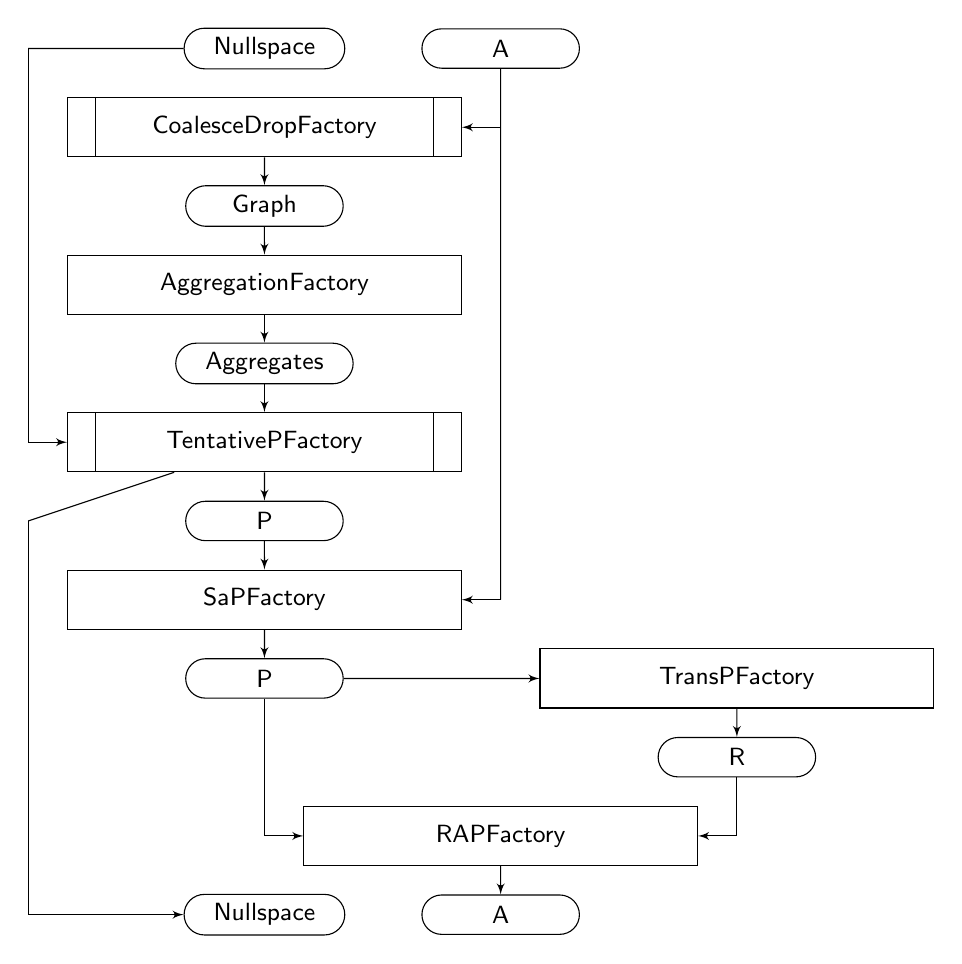
\begin{tikzpicture}[>=latex',font={\sf \small}]
\def\datawidth{2cm}
\def\dataheight{0.5cm}
\def\factorywidth{5cm}
\def\factoryheight{0.75cm}

\node(A) at (3,1) [draw, terminal, minimum width=\datawidth, minimum height=\dataheight]{A};
\node(Nullspace) at (0,1) [draw, terminal, minimum width=\datawidth, minimum height=\dataheight]{Nullspace};
\coordinate (co1) at (-3,1);
\coordinate (co2) at (-3,-4);
\coordinate (co3) at (3,-6);
\coordinate (co4) at (-3,-5);
\node(CoalesceDropFactory) at (0,0) [draw, predproc, minimum width=\factorywidth, minimum height=\factoryheight]{CoalesceDropFactory};
\node(Graph) at (0,-1) [draw, terminal, minimum width=\datawidth, minimum height=\dataheight]{Graph};
\node(AggregationFactory) at (0,-2) [draw, process, minimum width=\factorywidth, minimum height=\factoryheight]{AggregationFactory};
\node(Aggregates) at (0,-3) [draw, terminal, minimum width=\datawidth, minimum height=\dataheight]{Aggregates};
\node(TentativePFactory) at (0,-4) [draw, predproc, minimum width=\factorywidth, minimum height=\factoryheight]{TentativePFactory};
\node(Ptent) at (0,-5) [draw, terminal, minimum width=\datawidth, minimum height=\dataheight]{P};
\node(SaPFactory) at (0,-6) [draw, process, minimum width=\factorywidth, minimum height=\factoryheight]{SaPFactory};
\node(P) at (0,-7) [draw, terminal, minimum width=\datawidth, minimum height=\dataheight]{P};
\node(TransPFactory) at (6,-7) [draw, process, minimum width=\factorywidth, minimum height=\factoryheight]{TransPFactory};
\node(R) at (6,-8) [draw, terminal, minimum width=\datawidth, minimum height=\dataheight]{R};
\node(RAPFactory) at (3,-9) [draw, process, minimum width=\factorywidth, minimum height=\factoryheight]{RAPFactory};
\node(A2) at (3,-10) [draw, terminal, minimum width=\datawidth, minimum height=\dataheight]{A};
\node(Nullspace2) at (0,-10) [draw, terminal, minimum width=\datawidth, minimum height=\dataheight]{Nullspace};
\draw[-] (Nullspace) -- (co1);
\draw[-] (co1) -- (co2);
\draw[->] (co2) -- (TentativePFactory);
\draw[->] (A) |- (CoalesceDropFactory);
\draw[->] (CoalesceDropFactory) -- (Graph);
\draw[->] (Graph) -- (AggregationFactory);
\draw[->] (AggregationFactory) -- (Aggregates);
\draw[->] (Aggregates) -- (TentativePFactory);
\draw[-]  (A) -- (co3);
\draw[->] (co3) -- (SaPFactory);
\draw[->] (TentativePFactory) -- (Ptent);
\draw[->] (Ptent) -- (SaPFactory);
\draw[->] (SaPFactory) -- (P);
\draw[->] (P) |- (RAPFactory);
\draw[->] (P) -- (TransPFactory);
\draw[->] (TransPFactory) -- (R);
\draw[->] (R) |- (RAPFactory);
\draw[-]  (TentativePFactory) -- (co4);
\draw[->] (co4) |- (Nullspace2);
\draw[->] (RAPFactory) -- (A2);
\end{tikzpicture}
\caption{General workflow for smoothed aggregation transfer operators and Galerkin product}
\label{fig:generalworkflow}
\end{figure}

In figure \ref{fig:generalworkflow} we show the process of generating smoothed aggregation transfer operators. We start with an approximation of the fine level null space and the fine level matrix $A$. 
First, the \textit{CoalesceDropFactory} builds the graph of the fine level matrix $A$. If requested by the user it is possible to apply some filtering strategy to the fine level matrix before the graph is built. The graph of matrix $A$ is then used to build aggregates. The fine level null space together with the aggregation information is needed to define the non-smoothed tentative prolongation operator with the \textit{TentativePFactory}. Be aware that there are some more connections between the \textit{CoalesceDropFactory} and the \textit{TentativePFactory}, which are not shown here for simplicity. In case of not just one DOF per node, the \textit{CoalesceDropFactory} makes use of a helper class \textit{AmalgamationFactory} which amalgamates the matrix for finding the amalgamated graph. The hidden \textit{AmalgamationFactory} provides some information which is used in the \textit{TentativePFactory} to reconstruct the unamalgamated transfer operators from the amalgamated aggregation information. More details follow in other tutorials with vector problems instead of scalar problems.

Note, that the \textit{TentativePFactory} both generates the non-smoothed tentative transfer operator as well as the coarse level null space. Once the tentative prolongation operator is built, it is smoothed using the \textit{SaPFactory}. The \textit{TransPFacotry} builds the restriction operator just by transposing the smoothed prolongation operator. Finally, the \textit{RAPFactory} builds the coarse level matrix $A$.

Alltogether, the algorithm ends with an approximation of the coarse level null space and a coarse matrix $A$.


\section{Tutorial 2}

\subsection{Test example}
We generate a test matrix corresponding to the stencil of a 2D Laplacian operator on a structured Cartesian grid. The matrix stencil is
\begin{displaymath}
\frac{1}{h^2}\begin{pmatrix} & -1 & \\ -1 & 4 & -1 \\ & -1 & \end{pmatrix}.
\end{displaymath}
The resulting matrix is symmetric positive definite. We choose the right hand side to be the constant vector one and use a random initial guess for the iterative solution process. The problem domain is the unit cube with a Cartesian (uniform) mesh.

\subsection{Test program}

\subsection{XML Interface}

\begin{Listing} 
\begin{center} 
\begin{lstlisting}[language=XML,label=listing:SAAMGXML]
<ParameterList name="MueLu">
  <ParameterList name="Matrix">
    <Parameter name="PDE equations" type="int" value="1"/> 
  </ParameterList>

  <!-- Factory collection -->
  <ParameterList name="Factories">
     
    <ParameterList name="myJacobi">
      <Parameter name="factory" type="string" value="TrilinosSmoother"/>
      <Parameter name="type" type="string" value="RELAXATION"/>
      <ParameterList name="ParameterList">
       <Parameter name="relaxation: type" type="string" value="Jacobi"/>
       <Parameter name="relaxation: sweeps" type="int"    value="1"/>
       <Parameter name="relaxation: damping factor" type="double" value="0.9"/>
      </ParameterList>
    </ParameterList>
   </ParameterList>

  <!-- Definition of the multigrid preconditioner -->
  <ParameterList name="Hierarchy">

    <Parameter name="numDesiredLevel" type="int" value="1"/> 
    <Parameter name="maxCoarseSize" type="int" value="10"/>
    <Parameter name="verbosity" type="string"   value="Low"/>

    <ParameterList name="AllButCoarsestLevel">
      <Parameter name="startLevel" type="int" value="0"/>
      <Parameter name="Smoother" type="string" value="myJacobi"/>
    </ParameterList>

    <ParameterList name="CoarsestLevel">
     <Parameter name="CoarseSolver" type="string"   value="myJacobi"/>    
    </ParameterList>
  </ParameterList>
</ParameterList>
\end{lstlisting}
\caption{Structure of XML input file for \MueLu~ with smoothed aggregation transfer operators and Jacobi level smoothers.} 
\label{listing:SAAMGXML}
\end{center}
\end{Listing}

\paragraph{Step 1: Start with one-level method.}
Before we apply a multigrid method as solver, let's start with simple Jacobi sweeps and have a look at the error.
By setting the maximum multigrid levels to 1 and using a Jacobi smoother as coarse solver we obtain a pseudo multigrid method which corresponds to a simple Jacobi iteration. Listing \ref{listing:SAAMGXML} gives the multigrid XML parameters for the 1 level dummy multigrid method. Figures \ref{fig:2dlap111} to \ref{fig:2dlap11100} as well as figures \ref{fig:2dlap511} to \ref{fig:2dlap51100} show the smoothing effect of the Jacobi iteration.

\begin{graybox}
 \textbf{Exercise}
 \begin{itemize}
 \item Run the test program using the solver parameters from listing% \ref{listing:SAAMGXML}.
       \begin{verbatim}
       ./MueLu_laplace2d.exe --xml=xml/s2a.xml
       \end{verbatim}
       Note, that \verb|./MueLu_laplace2d.exe --help| prints all available options. Use \verb|mpirun| to run the program in parallel, e.g. on 2 processors
       \begin{verbatim}
       mpirun -np 2 ./MueLu_laplace2d.exe --xml=xml/s2a.xml
       \end{verbatim}
 \item For visualization of the output use the \verb|hands-on.sh| script. Run the script with
       \begin{verbatim}
       ./hands-on.sh
       \end{verbatim}
       and choose option 1 for the 2D Laplace example on a $50\times 50$ mesh. Then, the output is
       \begin{verbatim}
=== 2D Laplace (50 x 50) === 

 solver: procs: 2 Multigrid sweeps: 1


1) rerun example              7) plot exact solution
2) change multigrid sweeps    8) plot Multigrid solution
3) change mesh                9) plot error
4) change solver             10) plot proc distribution
5) change procs              11) Quit
6) show output
       \end{verbatim}
       Select option 6 to print the output of the \verb|MueLu_laplace2d.exe| program on screen. With \verb|q| you return to above menu. Option 7 plots the exact solution, that has been calculated with a direct solver. Option 8 plots the approximate solution after one sweep with the multigrid V cycle. Option 9 plots the error (the difference of the exact solution and the approximate multigrid solution).
 \end{itemize}
 \end{graybox}

\paragraph{Step 2: Increase number of multigrid levels.}
The next step is to increase the number of multigrid levels. We begin with a 2 level multigrid method. We choose the parameters \texttt{numDesiredLevel} \texttt{maxCoarseSize} accordingly such that a 2 level multigrid hierarchy is built. The parameter \texttt{maxCoarseSize} defines the size of the coarse level problem (number of matrix rows of the coarsest system) before the multigrid coarsening is stopped. Again we use Jacobi iterations as level smoothers on all multigrid levels with a fixed damping parameter $\omega=0.9$.
As one can see from figures  \ref{fig:2dlap121} to \ref{fig:2dlap12100} the error is reduced more efficiently when using more multigrid levels. A too high number of level smoothing sweeps with Jacobi gives no significant improvement.

\begin{graybox}
 \textbf{Exercise}
 \begin{itemize}
  \item Create a copy of the xml solver parameters in file \verb|xml/s2a.xml|, that you can adapt for your experiments.
        \begin{verbatim}
        cp xml/s2a.xml mysolver.xml
        \end{verbatim}
  \item Run the \verb|hands-on.sh| script, select option 1 for the 2D Laplace example. Then choose option 4 to change the used solver parameters and enter your chosen filename for your solver parameters file.
        \begin{verbatim}
=== 2D Laplace (50 x 50) === 

 solver: procs: 2 Multigrid sweeps: 1
 
1) rerun example              7) plot exact solution
2) change multigrid sweeps    8) plot Multigrid solution
3) change mesh                9) plot error
4) change solver             10) plot proc distribution
5) change procs              11) Quit
6) show output
Select: 4

*** 2D Laplace example ***

XML file=mysolver.xml
        \end{verbatim}
        The filename for the currently used solver parameters is also printed above the menu, such that you can check which solver parameter file is used.
   \item Edit your solver parameter file (e.g. \verb|mysolver.xml|) using your favorite text editor and adapt the parameters. Set the \texttt{numDesiredLevel} parameter to $2$ to obtain a two level multigrid method and choose a value for \texttt{maxCoarseSize} that is small enough that a 2 level multigrid hierarchy is built (e.g. 10). Don't forget to save your changes.
   \item Select the option 1 to rerun your example using the solver parameters from \verb|mysolver.xml| with your recent changes. Check the solver output and the plots. You can also increase the number of multigrid sweeps (using option 2) and see how the error changes.
%   \item Change your solver parameters for obtaining a three level multigrid method.
 \end{itemize}
\end{graybox}

\paragraph{Step 3: Use a direct solver on the coarsest grid.}
One of the core ideas of multigrid is to coarsen the fine level problem such that we can use a direct solver to obtain the exact coarse level solution with reasonable costs. In the \texttt{CoarsestLevel} section we change the value of the parameter \texttt{CoarseSolver} to \textit{DirectSolver}. That is, we use Jacobi sweeps as pre- and postsmoother on the finest and the intermedium levels and a direct solve on the coarsest level.
In figures \ref{fig:jacobisolver} and \ref{fig:directsolver} one can compare the output of the multigrid setup either when using Jacobi sweeps as coarse level smoothers or a direct solver. One can also see, that a direct solver has some beneficial effects when the multigrid method is used as preconditioner within CG. The number of linear iterations is reduced from 10 iterations to 7 iterations.

\begin{graybox}
 \textbf{Exercise}
 \begin{itemize}
  \item Run the \verb|hands-on.sh| script, select option 1 for the 2D Laplace example. Then choose option 4 to change the used solver parameters and enter your chosen filename for your solver parameters file.
  \item Change your solver parameters for obtaining a three level multigrid method. Furthermore change the parameter \verb|CoarseSolver| in the \verb|CoarsestLevel| section from \verb|myJacobi| to \verb|DirectSolver|. Then, on the coarsest level a direct solver is used (KLU) instead of the Jacobi sweep defined in the \verb|myJacobi| section. Don't forget to save your changes and to rerun the example.    
  \item Check the difference in the output of the multigrid setup.
 \end{itemize}
\end{graybox}

\begin{figure}
\tiny
\begin{minipage}{\textwidth}
\begin{verbatim}
 --------------------------------------------------------------------------------
 ---                            Multigrid Summary                             ---
 --------------------------------------------------------------------------------
 Number of levels    = 3
 Operator complexity = 1.36
 Max Coarse Size     = 10
 Implicit Transpose  = false
 
 matrix rows    nnz  nnz/row procs
 A 0    2500  12300     4.92  2
 A 1     442   3870     8.76  2
 A 2      60    520     8.67  2
 
 Smoother (level 0) both : MueLu::IfpackSmoother{type = point relaxation stand-alone}
 
 Smoother (level 1) both : MueLu::IfpackSmoother{type = point relaxation stand-alone}
 
 Smoother (level 2) pre  : MueLu::IfpackSmoother{type = point relaxation stand-alone}
 Smoother (level 2) post :  no smoother
 
Use multigrid hierarchy as preconditioner within CG.

                *******************************************************
                ***** Problem: Epetra::CrsMatrix
                ***** Preconditioned CG solution
                ***** MueLu::Hierarchy
                ***** No scaling
                *******************************************************

                iter:    0           residual = 1.000000e+00
                iter:    1           residual = 1.412917e-02
                iter:    2           residual = 1.015400e-03
                iter:    3           residual = 5.716660e-04
                iter:    4           residual = 2.170943e-04
                iter:    5           residual = 3.271912e-05
                iter:    6           residual = 1.164732e-05
                iter:    7           residual = 2.172965e-06
                iter:    8           residual = 3.257416e-07
                iter:    9           residual = 2.669124e-08
                iter:   10           residual = 4.527172e-09


                Solution time: 0.017486 (sec.)
                total iterations: 10
\end{verbatim}
\end{minipage}
\caption{Multigrid Summary of setup phase for 3 level multigrid method with Jacobi level smoothers on all multigrid level. The multigrid method is used as preconditioner within a CG method for solving the 2D Laplace equation on the $50\times 50$ mesh.}
\label{fig:jacobisolver}
\end{figure}

\begin{figure}
\tiny
\begin{minipage}{\textwidth}
\begin{verbatim}
 --------------------------------------------------------------------------------
 ---                            Multigrid Summary                             ---
 --------------------------------------------------------------------------------
 Number of levels    = 3
 Operator complexity = 1.36
 Max Coarse Size     = 10
 Implicit Transpose  = false
 
 matrix rows    nnz  nnz/row procs
 A 0    2500  12300     4.92  2
 A 1     442   3870     8.76  2
 A 2      60    520     8.67  2
 
 Smoother (level 0) both : MueLu::IfpackSmoother{type = point relaxation stand-alone}
 
 Smoother (level 1) both : MueLu::IfpackSmoother{type = point relaxation stand-alone}
 
 Smoother (level 2) pre  : MueLu::AmesosSmoother{type = Klu}
 Smoother (level 2) post :  no smoother
 
 Use multigrid hierarchy as preconditioner within CG.

                *******************************************************
                ***** Problem: Epetra::CrsMatrix
                ***** Preconditioned CG solution
                ***** MueLu::Hierarchy
                ***** No scaling
                *******************************************************

                iter:    0           residual = 1.000000e+00
                iter:    1           residual = 1.413569e-02
                iter:    2           residual = 9.769450e-04
                iter:    3           residual = 7.720818e-05
                iter:    4           residual = 6.184216e-06
                iter:    5           residual = 4.067740e-07
                iter:    6           residual = 4.135880e-08
                iter:    7           residual = 2.756129e-09


                Solution time: 0.012708 (sec.)
                total iterations: 7
\end{verbatim}
\end{minipage}
\caption{Multigrid Summary of setup phase for 3 level multigrid method with direct solver KLU on the coarsest level. The multigrid method is used as preconditioner within a CG method for solving the 2D Laplace equation on the $50\times 50$ mesh.}
\label{fig:directsolver}
\end{figure}

\begin{figure}
\subfigure[1 level with 1 Jacobi sweep ($\omega=0.9$)\label{fig:2dlap111}]{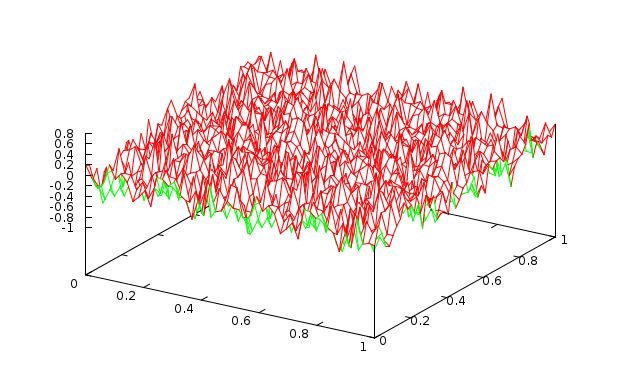
\includegraphics[width=0.3\textwidth]{images/1level_1jac09.png}}\hspace{0.03\textwidth}
\subfigure[1 level with 10 Jacobi sweeps ($\omega=0.9$)\label{fig:2dlap1110}]{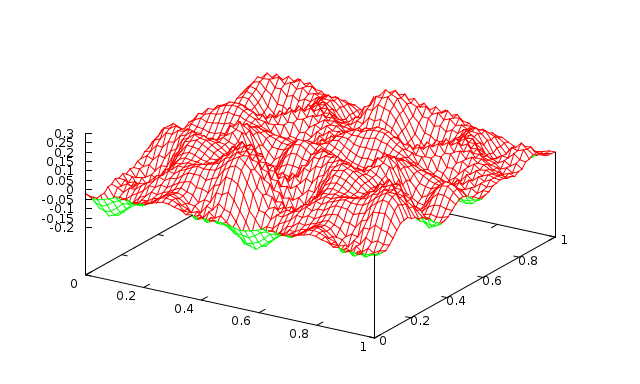
\includegraphics[width=0.3\textwidth]{images/1level_10jac09.png}}\hspace{0.03\textwidth}
\subfigure[1 level with 100 Jacobi sweeps ($\omega=0.9$)\label{fig:2dlap11100}]{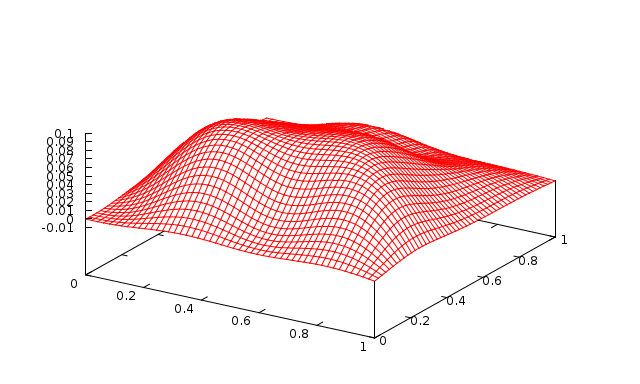
\includegraphics[width=0.3\textwidth]{images/1level_100jac09.png}} \\
\subfigure[2 level with 1 Jacobi sweep ($\omega=0.9$)\label{fig:2dlap121}]{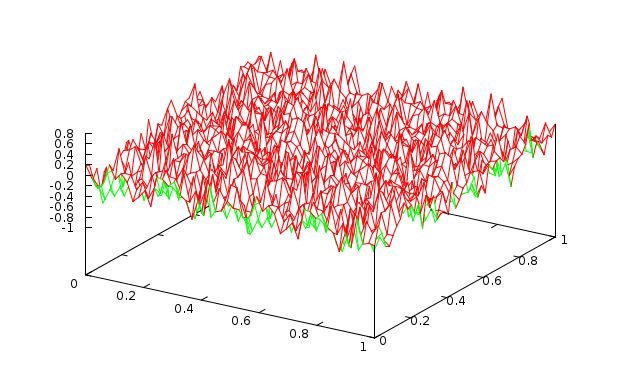
\includegraphics[width=0.3\textwidth]{images/2level_1jac09.png}}\hspace{0.03\textwidth}
\subfigure[2 level with 10 Jacobi sweeps ($\omega=0.9$)\label{fig:2dlap1210}]{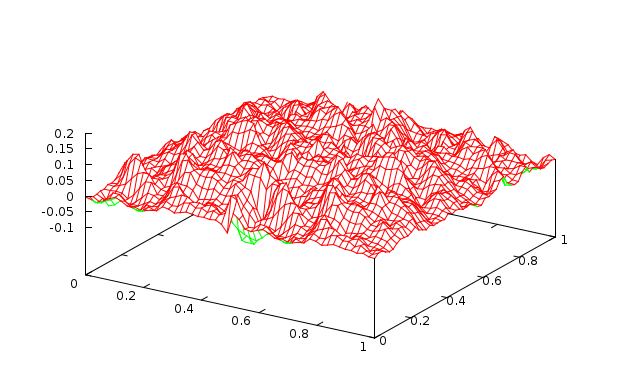
\includegraphics[width=0.3\textwidth]{images/2level_10jac09.png}}\hspace{0.03\textwidth}
\subfigure[2 level with 100 Jacobi sweeps ($\omega=0.9$)\label{fig:2dlap12100}]{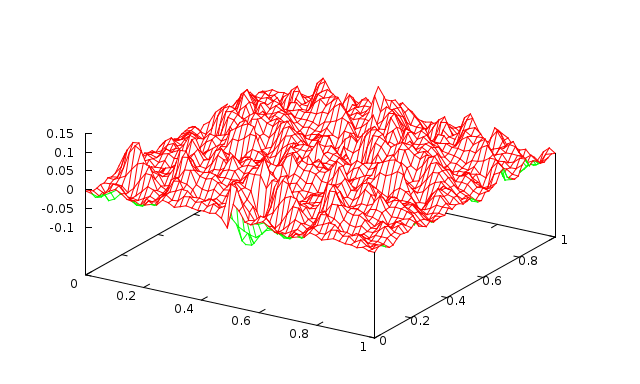
\includegraphics[width=0.3\textwidth]{images/2level_100jac09.png}} \\
\subfigure[3 level with 1 Jacobi sweep ($\omega=0.9$)\label{fig:2dlap131}]{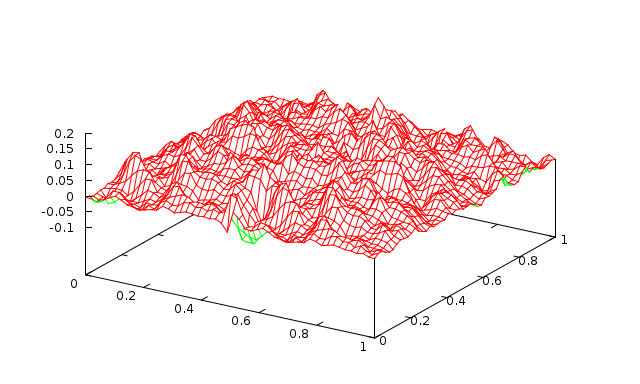
\includegraphics[width=0.3\textwidth]{images/3level_1jac09.png}}\hspace{0.03\textwidth}
\subfigure[3 level with 10 Jacobi sweeps ($\omega=0.9$)\label{fig:2dlap1310}]{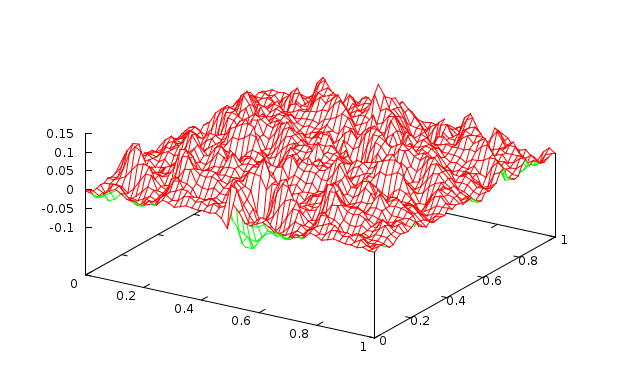
\includegraphics[width=0.3\textwidth]{images/3level_10jac09.png}}\hspace{0.03\textwidth}
\subfigure[3 level with 100 Jacobi sweeps ($\omega=0.9$)\label{fig:2dlap13100}]{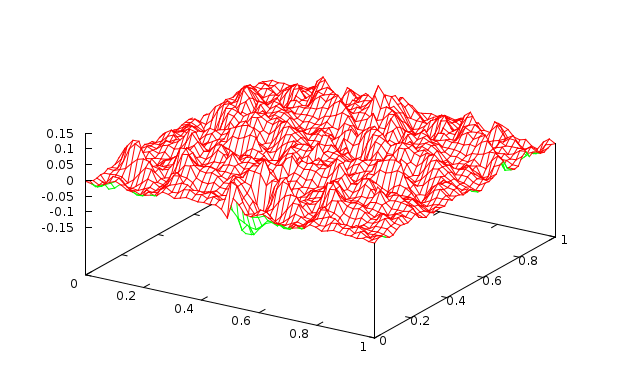
\includegraphics[width=0.3\textwidth]{images/3level_100jac09.png}} \\
\caption{2D Laplace equation on $50\times 50$ mesh after 1 V-cycle with an AMG multigrid solver and Jacobi smoothers on all multigrid levels. (2 processors)}
\end{figure}


\begin{figure}
\subfigure[1 level with 1 Jacobi sweep ($\omega=0.9$)\label{fig:2dlap511}]{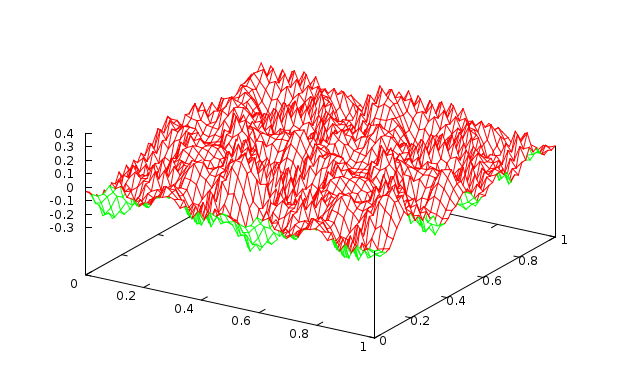
\includegraphics[width=0.3\textwidth]{images/5sweeps_1level_1jac09.png}}\hspace{0.03\textwidth}
\subfigure[1 level with 10 Jacobi sweeps ($\omega=0.9$)\label{fig:2dlap5110}]{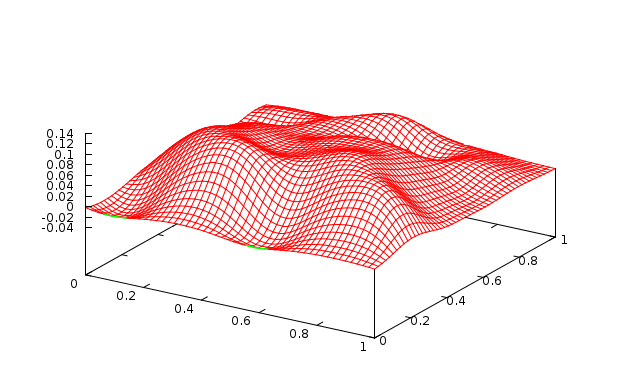
\includegraphics[width=0.3\textwidth]{images/5sweeps_1level_10jac09.png}}\hspace{0.03\textwidth}
\subfigure[1 level with 100 Jacobi sweeps ($\omega=0.9$)\label{fig:2dlap51100}]{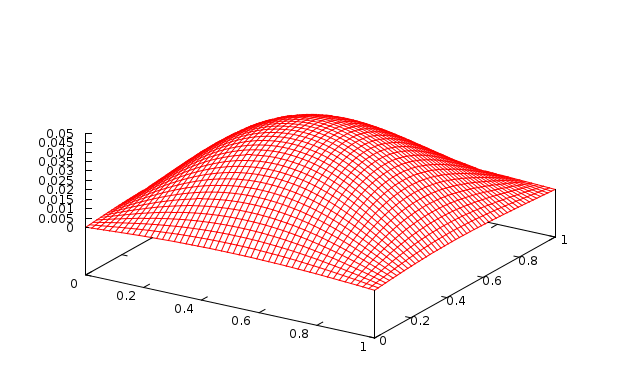
\includegraphics[width=0.3\textwidth]{images/5sweeps_1level_100jac09.png}} \\
\subfigure[2 level with 1 Jacobi sweep ($\omega=0.9$)\label{fig:2dlap521}]{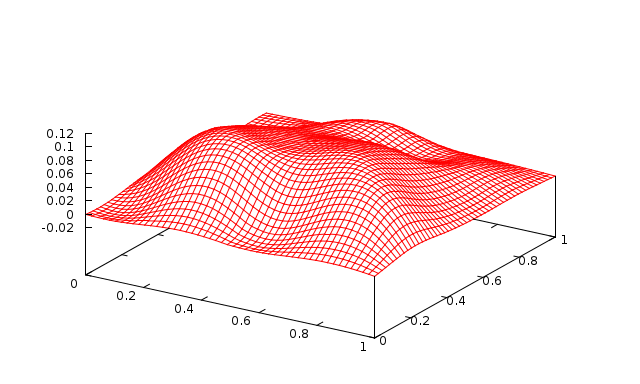
\includegraphics[width=0.3\textwidth]{images/5sweeps_2level_1jac09.png}}\hspace{0.03\textwidth}
\subfigure[2 level with 10 Jacobi sweeps ($\omega=0.9$)\label{fig:2dlap5210}]{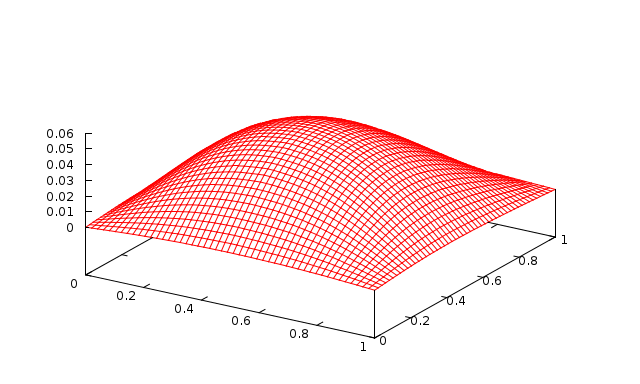
\includegraphics[width=0.3\textwidth]{images/5sweeps_2level_10jac09.png}}\hspace{0.03\textwidth}
\subfigure[2 level with 100 Jacobi sweeps ($\omega=0.9$)\label{fig:2dlap52100}]{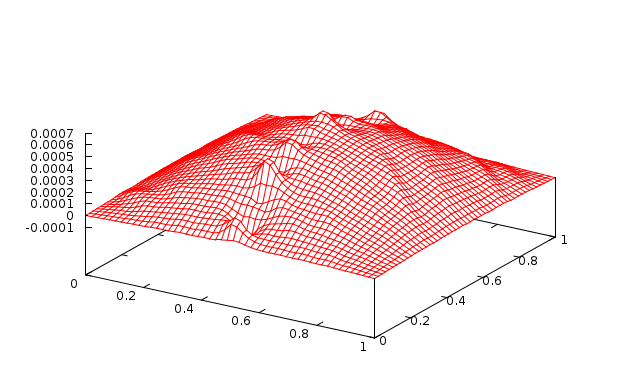
\includegraphics[width=0.3\textwidth]{images/5sweeps_2level_100jac09.png}} \\
\subfigure[3 level with 1 Jacobi sweep ($\omega=0.9$)\label{fig:2dlap531}]{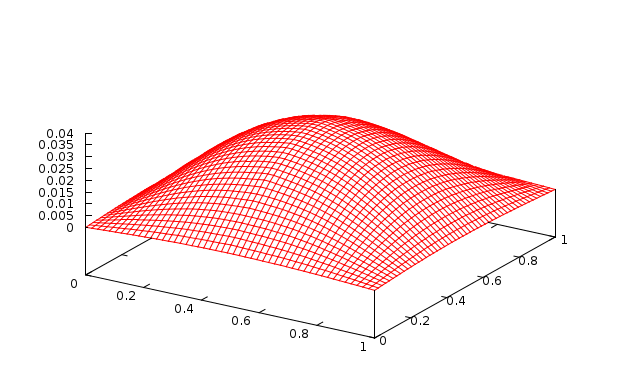
\includegraphics[width=0.3\textwidth]{images/5sweeps_3level_1jac09.png}}\hspace{0.03\textwidth}
\subfigure[3 level with 10 Jacobi sweeps ($\omega=0.9$)\label{fig:2dlap5310}]{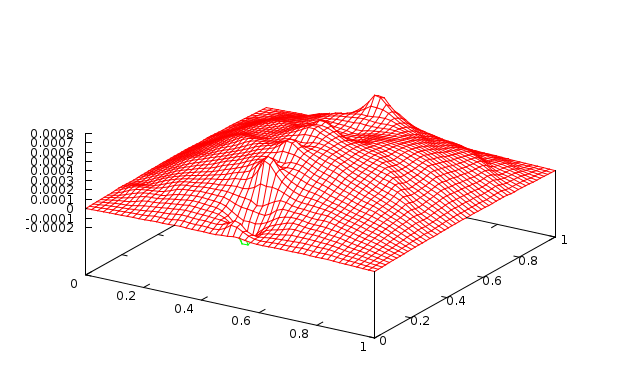
\includegraphics[width=0.3\textwidth]{images/5sweeps_3level_10jac09.png}}\hspace{0.03\textwidth}
\subfigure[3 level with 100 Jacobi sweeps ($\omega=0.9$)\label{fig:2dlap53100}]{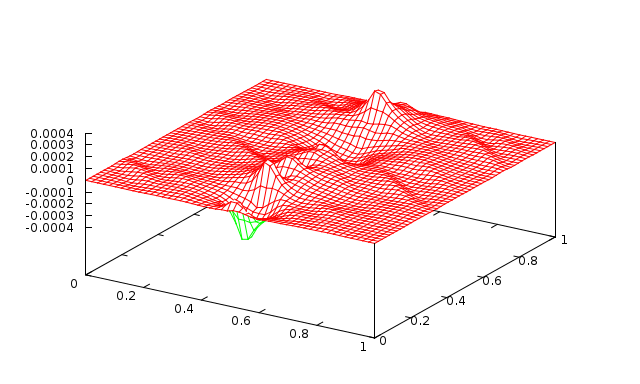
\includegraphics[width=0.3\textwidth]{images/5sweeps_3level_100jac09.png}} \\
\caption{2D Laplace equation on $50\times 50$ mesh after 5 V-cycle with an AMG multigrid solver and Jacobi smoothers on all multigrid levels. (2 processors)}
\end{figure}

\paragraph{Step 4: Use better level smoothers.}
The Jacobi iteration might be a very cheap and fully parallel level smoother, but often one obtains better results when using more expensive and better level smoothers.
In the example XML files there are sections for many possible level smoothers, such that polynomial smoothers (Chebyshev) as well as Gauss-Seidel variants. Usually a small number of smoothing sweeps (e.g. 1 - 5) is sufficient for smoothing the high frequency error without too high costs. More challenging is to find a proper choice for the damping parameters which are highly problem dependent.

\begin{graybox}
 \textbf{Exercise}
 \begin{itemize}
  \item In the xml paramter file \verb|xml/s2b.xml| you can find the definition of some other types of multigrid level smoothers, such as Chebyshev, Jacobi and different Gauss-Seidel variants.
  \item Run the \verb|hands-on.sh| script for the 2D Laplace example and use the \verb|xml/s2b.xml| solver file. Change the \verb|Smoother| parameter in the \verb|AllButCoarsestLevel| section from \verb|myJacobi| to some other smoother that is defined in the \verb|Factories| section, e.g. \verb|SymGaussSeidel|.
  \item Play around with different level smoothers and smoother parameters.
 \end{itemize}
\end{graybox}


\section{Tutorial 3}

\subsection{Test example}
The \texttt{Recirc2D} example uses a matrix corresponding to the finite-difference discretization of the problem
\begin{displaymath}
-\varepsilon\Delta u + (v_x,v_y)\cdot \nabla u=f
\end{displaymath}
on the unit square, with $\varepsilon=1e-5$ and homogeneous Dirichlet boundary conditions. It is $v_x=4x(x-1)(1-2y)$ and $v_y=-4y(y-1)(1-2x)$.
The right hand side vector $f$ is chosen to be the constant vector 1. Due to the convective term the resulting linear system is non-symmetric and therefore more challenging for the iterative solver. The multigrid algorithm has to be adapted to the non-symmetry to obtain good convergence behaviour.

\subsection{Test program}

\subsection{Multigrid setup phase}

Smoothed aggregation based algebraic multigrid methods originally have not been designed for non-symmetric linear systems. Inappropriately smoothed transfer operators may significantly detoriate the convergence rate or even break convergence completely. 

\paragraph{Non-smoothed transfer operators.}
Before we introduce smoothed aggregation methods for non-symmetric linear systems we first go back one step and demonstrate how to use non-smoothed transfer operators which are eligible for non-symmetric linear systems. Figure \ref{fig:simpledesignnonsmoothed} gives a simplified example how to build the coarse level matrix $A_c$ using the fine level matrix $A$ only. First, we "somehow" build aggregates using the information of the fine level matrix $A$. The aggregates are then used to build the tentative non-smoothed prolongation operator. The restrictor is just the transpose of the (tentative) prolongator and finally the coarse level matrix $A_c$ is calculated by the triple product $A_c=RAP$.

In figure \ref{fig:simpledesignsaamg} the \verb|SaPFactory| has been added after the \verb|TentativePFactory|. Therein the non-smoothed transfer operator from the \verb|TentativePFactory| is smoothed using information of the fine level matrix $A$. This transfer operator design is used per default when the user does not specify its own transfer operator design. The default settings are optimal for symmetric positive definite systems. However for our non-symmetric problem they might be problematic.

\begin{figure}
\subfigure[Non-smoothed aggregation based AMG\label{fig:simpledesignnonsmoothed}]{
\scalebox{0.5}{
\begin{tikzpicture}[>=latex',font={\sf \small}, node distance=2cm]
\def\datawidth{2cm}
\def\dataheight{0.5cm}
\def\factorywidth{4cm}
\def\factoryheight{0.75cm}
%\draw[help lines] (-10,-10) grid (10,10);
\begin{scope}[>=triangle 60]
\node(A) at (-3,10) [draw, terminal, minimum width=\datawidth, minimum height=\dataheight]{$A$};
\node(nothing) at (-3,8) [draw, process, minimum width=\factorywidth, minimum height=\factoryheight]{...};
\node [draw, process, minimum width=\factorywidth, minimum height=\factoryheight, below of=nothing] (AggregationFactory) {AggregationFactory};
\node [draw, process, minimum width=\factorywidth, minimum height=\factoryheight, below of=AggregationFactory] (TentativePFactory) {TentativePFactory};
\node [draw, process, minimum width=\factorywidth, minimum height=\factoryheight, right of=TentativePFactory,node distance=6cm] (TransPFactory) {TransPFactory};
\node [draw, process, minimum width=\factorywidth, minimum height=\factoryheight, below of=TentativePFactory] (RAPFactory) {RAPFactory};
\node(A2) at (-3,0) [draw, terminal, minimum width=\datawidth, minimum height=\dataheight]{$A_c$};
\draw[->] (A) -- (nothing);
\draw[->] (nothing) -- (AggregationFactory);
\draw[->] (A) to[out=180,in=180] node [near start, left] {} (TentativePFactory);
\draw[->] (A) to[out=180,in=180] node [near start, left] {} (RAPFactory);
\draw[->] (AggregationFactory) -- node [near start, left] {Aggregates} (TentativePFactory);
\draw[->] (TentativePFactory) -- node [near start, below] {P} (TransPFactory);
\draw[->] (TentativePFactory) -- node [near start, left] {P} (RAPFactory);
\draw[->] (TransPFactory) -- node [near start, below] {R} (RAPFactory);
\draw[->] (RAPFactory) -- node [near start, below] {} (A2);
\end{scope}
\end{tikzpicture}
} % end scalebox
} % end subfigure 1
\subfigure[Smoothed aggregation AMG (SA-AMG)\label{fig:simpledesignsaamg}]{
\scalebox{0.5}{
\begin{tikzpicture}[>=latex',font={\sf \small}, node distance=2cm]
\def\datawidth{2cm}
\def\dataheight{0.5cm}
\def\factorywidth{4cm}
\def\factoryheight{0.75cm}
%\draw[help lines] (-10,-10) grid (10,10);
\begin{scope}[>=triangle 60]
\node(A) at (-3,10) [draw, terminal, minimum width=\datawidth, minimum height=\dataheight]{$A$};
\node(nothing) at (-3,8) [draw, process, minimum width=\factorywidth, minimum height=\factoryheight]{...};
\node [draw, process, minimum width=\factorywidth, minimum height=\factoryheight, below of=nothing] (AggregationFactory) {AggregationFactory};
\node [draw, process, minimum width=\factorywidth, minimum height=\factoryheight, below of=AggregationFactory] (TentativePFactory) {TentativePFactory};
\node [draw, process, minimum width=\factorywidth, minimum height=\factoryheight, below of=TentativePFactory] (SaPFactory) {SaPFactory};
\node [draw, process, minimum width=\factorywidth, minimum height=\factoryheight, right of=SaPFactory,node distance=6cm] (TransPFactory) {TransPFactory};
\node [draw, process, minimum width=\factorywidth, minimum height=\factoryheight, below of=SaPFactory] (RAPFactory) {RAPFactory};
\node(A2) at (-3,-2) [draw, terminal, minimum width=\datawidth, minimum height=\dataheight]{$A_c$};
\draw[->] (A) -- (nothing);
\draw[->] (nothing) -- (AggregationFactory);
\draw[->] (A) to[out=180,in=180] node [near start, left] {} (TentativePFactory);
\draw[->] (A) to[out=180,in=180] node [near start, left] {} (SaPFactory);
\draw[->] (A) to[out=180,in=180] node [near start, left] {} (RAPFactory);
\draw[->] (AggregationFactory) -- node [near start, left] {Aggregates} (TentativePFactory);
\draw[->] (TentativePFactory) -- node [near start, left] {P} (SaPFactory);
\draw[->] (SaPFactory) -- node [near start, below] {P} (TransPFactory);
\draw[->] (SaPFactory) -- node [near start, left] {P} (RAPFactory);
\draw[->] (TransPFactory) -- node [near start, below] {R} (RAPFactory);
\draw[->] (RAPFactory) -- node [near start, below] {} (A2);
\end{scope}
\end{tikzpicture}
} % end scalebox
} % end subfigure 2
\caption{Simple factory design for aggregation based algebraic multigrid methods.}
\label{fig:simpledesign}
\end{figure}

\paragraph{Smoothed transfer operators for non-symmetric systems.}
In case of non-symmetric linear systems it is $A\neq A^T$. Therefore it is a bad idea just to use the transposed of the smoothed prolongation operator for the restrictor. Let $\widehat{P}$ be the non-smoothed tentative prolongation operator. Then the smoothed prolongation operator $P$ is built using
\begin{displaymath}
P = \bigl(I-\omega A\bigr) \widehat{P},
\end{displaymath}
with some reasonable smoothing parameter $\omega>0$.
The standard restrictor is 
\begin{displaymath}
R = P^T = \widehat{P}^T - \omega \widehat{P}^T A^T = \widehat{P}^T\bigl(I-\omega A^T\bigr).
\end{displaymath}
That is, the restrictor would be smoothed using the information of $A^T$. However, for non-symmetric systems we want to use the information of matrix $A$ for smoothing the restriction operator, too. The restriction operator shall we built by the formula
\begin{displaymath}
R = P^T = \widehat{P}^T - \omega \widehat{P}^T A.
\end{displaymath}
This corresponds to apply the same smoothing strategy to the non-smoothed restriction operator $\widehat{R}=\widehat{P}^T$ which is applied to the (tentative) prolongation operator with using $A^T$ as input instead of matrix $A$. Figure \ref{fig:simpledesignpgamg} shows the changed factory design. The dashed line denotes, that the same smoothing strategy is used than for the prolongation operator. The concept is known as Petrov-Galerkin smoothed aggregation approach in the literature.

\begin{figure}
\scalebox{0.5}{
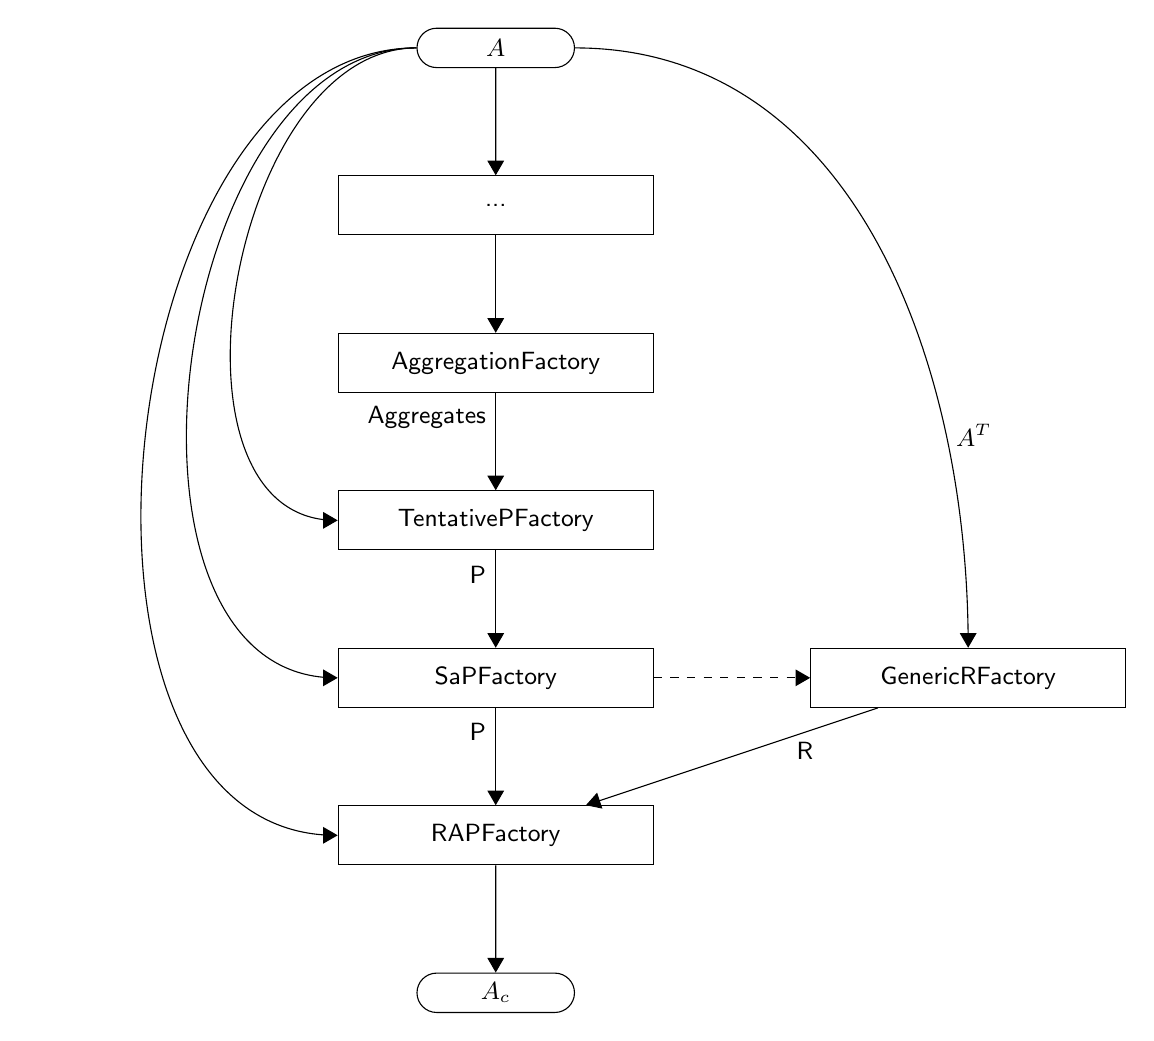
\begin{tikzpicture}[>=latex',font={\sf \small}, node distance=2cm]
\def\datawidth{2cm}
\def\dataheight{0.5cm}
\def\factorywidth{4cm}
\def\factoryheight{0.75cm}
%\draw[help lines] (-10,-10) grid (10,10);
\begin{scope}[>=triangle 60]
\node(A) at (-3,10) [draw, terminal, minimum width=\datawidth, minimum height=\dataheight]{$A$};
\node(nothing) at (-3,8) [draw, process, minimum width=\factorywidth, minimum height=\factoryheight]{...};
\node [draw, process, minimum width=\factorywidth, minimum height=\factoryheight, below of=nothing] (AggregationFactory) {AggregationFactory};
\node [draw, process, minimum width=\factorywidth, minimum height=\factoryheight, below of=AggregationFactory] (TentativePFactory) {TentativePFactory};
\node [draw, process, minimum width=\factorywidth, minimum height=\factoryheight, below of=TentativePFactory] (SaPFactory) {SaPFactory};
\node [draw, process, minimum width=\factorywidth, minimum height=\factoryheight, right of=SaPFactory,node distance=6cm] (GenericRFactory) {GenericRFactory};
\node [draw, process, minimum width=\factorywidth, minimum height=\factoryheight, below of=SaPFactory] (RAPFactory) {RAPFactory};
\node(A2) at (-3,-2) [draw, terminal, minimum width=\datawidth, minimum height=\dataheight]{$A_c$};
\draw[->] (A) -- (nothing);
\draw[->] (nothing) -- (AggregationFactory);
\draw[->] (A) to[out=180,in=180] node [near start, left] {} (TentativePFactory);
\draw[->] (A) to[out=180,in=180] node [near start, left] {} (SaPFactory);
\draw[->] (A) to[out=180,in=180] node [near start, left] {} (RAPFactory);
\draw[->] (A) to[out=0,in=90] node [near end, right] {$A^T$} (GenericRFactory);
\draw[->] (AggregationFactory) -- node [near start, left] {Aggregates} (TentativePFactory);
\draw[->] (TentativePFactory) -- node [near start, left] {P} (SaPFactory);
\draw[->,dashed] (SaPFactory) -- node [near start, below] {} (GenericRFactory);
\draw[->] (SaPFactory) -- node [near start, left] {P} (RAPFactory);
\draw[->] (GenericRFactory) -- node [near start, below] {R} (RAPFactory);
\draw[->] (RAPFactory) -- node [near start, below] {} (A2);
\end{scope}
\end{tikzpicture}
} % end scalebox
\caption{Simple factory design for smoothed aggregation based algebraic multigrid methods for non-symmetric systems.}
\label{fig:simpledesignpgamg}
\end{figure}



\subsection{XML Interface}

\paragraph{Non-smoothed transfer operators}

Listing \ref{listing:PAAMGXML} shows the parameters for non-smoothed transfer operators. The aggregates are built by the \verb|UncoupledAggregationFactory| which means that aggregates cannot overlap processor boundaries.

\begin{Listing} 
\begin{center} 
\begin{lstlisting}[language=XML,label=listing:PAXML]
<ParameterList name="MueLu">
  <!-- Factory collection -->
  <ParameterList name="Factories">
    <ParameterList name="UncoupledAggregationFact">
      <Parameter name="factory" type="string" value="UncoupledAggregationFactory"/>
      <Parameter name="Ordering" type="string" value="Natural"/>
      <Parameter name="MinNodesPerAggregate" type="int" value="4"/>
    </ParameterList>   
    <ParameterList name="myTentativePFact">
     <Parameter name="factory" type="string" value="TentativePFactory"/>
    </ParameterList>
    <ParameterList name="myRestrictorFact">
     <Parameter name="factory" type="string" value="TransPFactory"/>
     <Parameter name="P" type="string" value="myTentativePFact"/>
    </ParameterList>
  </ParameterList>

  <!-- Definition of the multigrid preconditioner -->
  <ParameterList name="Hierarchy">
    <Parameter name="numDesiredLevel" type="int" value="10"/>
    <Parameter name="maxCoarseSize" type="int" value="10"/>
    <Parameter name="verbosity" type="string" value="High"/>
    <ParameterList name="AllButCoarsestLevel">
      <Parameter name="startLevel" type="int"      value="0"/>
      <Parameter name="Aggregates" type="string"   value="UncoupledAggregationFact"/>
      <Parameter name="Nullspace" type="string"   value="myTentativePFact"/>
      <Parameter name="P" type="string"   value="myTentativePFact"/>
      <Parameter name="R" type="string"   value="myRestrictorFact"/>
    </ParameterList>
    <ParameterList name="CoarsestLevel">
      <Parameter name="CoarseSolver" type="string"   value="DirectSolver"/>
    </ParameterList>
  </ParameterList>
</ParameterList>
\end{lstlisting}
\caption{Structure of XML input file for \MueLu~ with non-smoothed aggregation transfer operators.} 
\label{listing:PAAMGXML}
\end{center}
\end{Listing}

In figure \ref{fig:ucoutput} a typical output (verbosity level "High") for \MueLu~ with uncoupled aggregation and non-smoothed transfer operators is shown as it is defined in the parameter list in listing \ref{listing:PAAMGXML} and shown in figure \ref{fig:simpledesignnonsmoothed}.
\begin{figure}
\tiny
\begin{verbatim}
 Build (MueLu::TentativePFactory)
  Build (MueLu::UncoupledAggregationFactory)
   Build (MueLu::CoalesceDropFactory)
    lightweight wrap = 0
    CoalesceDropFactory::Build(): found blockdim=1 from strided maps. offset=0
    Build (MueLu::AmalgamationFactory)
     AmalagamationFactory::Build(): found fullblocksize=1 and stridedblocksize=1 from strided maps. offset=0
    CoalesceDropFactory::SetupAmalgamationData() # of amalgamated blocks=2500
    CoalesceDropFactory: nodeMap 1250/2500 elements
   BuildAggregates (MueLu::OnePtAggregationAlgorithm)
    Aggregation (UC): Phase 0 (1pt aggregates): Nodes aggregated = 0 out of 2500 nodes
    Aggregation (UC): Phase 0 (1pt aggregates): Total aggregates = 0
    Aggregation (UC): Phase 0 (1pt aggregates): (WARNING) 2500 unaggregated nodes left
   BuildAggregates (MueLu::UncoupledAggregationAlgorithm)
    Aggregation (UC): UncoupledAggregationAlgorithm: Nodes aggregated = 2116 out of 2500 nodes
    Aggregation (UC): UncoupledAggregationAlgorithm: Total aggregates = 442
    Aggregation (UC): UncoupledAggregationAlgorithm: (WARNING) 384 unaggregated nodes left
   BuildAggregates (MueLu::MaxLinkAggregationAlgorithm)
    Aggregation (UC): Phase 2 (max_link, extend aggregates): Nodes aggregated = 2500 out of 2500 nodes
    Aggregation (UC): Phase 2 (max_link, extend aggregates): Total aggregates = 442
   BuildAggregates (MueLu::IsolatedNodeAggregationAlgorithm)
    Aggregation (UC): Phase 4 (isolated node aggregation): Nodes aggregated = 2500 out of 2500 nodes
    Aggregation (UC): Phase 4 (isolated node aggregation): Total aggregates = 442
   BuildAggregates (MueLu::EmergencyAggregationAlgorithm)
    Aggregation (UC): Phase 3 (emergency aggregation): Nodes aggregated = 2500 out of 2500 nodes
    Aggregation (UC): Phase 3 (emergency aggregation): Total aggregates = 442
   "UC": MueLu::Aggregates{nGlobalAggregates = 442}
  Build (MueLu::CoarseMapFactory)
   domainGIDOffset: 0 block size: 1 stridedBlockId: -1
  TentativePFactory : aggregates do not cross process boundaries
  Ptent size =  2500 x 442, nnz = 2500
  Ptent Load balancing info:
  Ptent   # active processes: 2,  # processes with data = 2
  Ptent   # rows per proc   : avg = 1.25e+03,  dev =  0.0%,  min =  +0.0%,  max =  +0.0%
  Ptent   #  nnz per proc   : avg = 1.25e+03,  dev =  0.0%,  min =  +0.0%,  max =  +0.0%
 Transpose P (MueLu::TransPFactory)
 Computing Ac (MueLu::RAPFactory)
  MxM: A x P
   ****** USING ML's MATRIX MATRIX MULTIPLY (LNM version) ******
  MxM: R x (AP) (explicit)
   ****** USING ML's MATRIX MATRIX MULTIPLY (LNM version) ******
  Ac size =  442 x 442, nnz = 2892
  Ac Load balancing info:
  Ac   # active processes: 2,  # processes with data = 2
  Ac   # rows per proc   : avg = 2.21e+02,  dev =  0.0%,  min =  +0.0%,  max =  +0.0%
  Ac   #  nnz per proc   : avg = 1.45e+03,  dev =  0.0%,  min =  +0.0%,  max =  +0.0%
\end{verbatim}
\caption{Exemplary output of \MueLu~ when generating the coarse level matrix $A_c$ using non-smoothed prolongation and restriction operators and uncoupled aggregation.}
\label{fig:ucoutput}
\end{figure}

\begin{graybox}
 \textbf{Exercise}
 \begin{itemize}
  \item Run the \verb|hands-on.sh| script for the 2D Recirc example and use the \verb|xml/s3a.xml| solver file. The \verb|xml/s3a.xml| contains non-smoothed transfer operators, a Jacobi smoother and a symmetric GaussSeidel smoother. Find reasonable smoother settings.
  \item Try different values for the \verb|MinNodesPerAggregate| parameter. The parameter defines the minimum size of nodes of each aggregate. How does the multigrid setup differ when using a small value (e.g. 3), a value in the medium range (e.g. 6) and a big value (e.g. 12)?
 \end{itemize}
\end{graybox}

Choosing \verb|MinNodesPerAggregate|$=4$ we obtain a 4 level multigrid method:
{\footnotesize
\begin{verbatim}
 --------------------------------------------------------------------------------
 ---                            Multigrid Summary                             ---
 --------------------------------------------------------------------------------
 Number of levels    = 4
 Operator complexity = 1.27
 Max Coarse Size     = 10
 Implicit Transpose  = false
 
 matrix rows    nnz  nnz/row procs
 A 0    2500  12300     4.92  2
 A 1     442   2892     6.54  2
 A 2      60    348     5.80  2
 A 3      10     46     4.60  2
\end{verbatim}}

When using \verb|MinNodesPerAggregate|$=9$ the multigrid setup routine produces a 6 level multigrid method
{\footnotesize
\begin{verbatim}
 --------------------------------------------------------------------------------
 ---                            Multigrid Summary                             ---
 --------------------------------------------------------------------------------
 Number of levels    = 6
 Operator complexity = 1.92
 Max Coarse Size     = 10
 Implicit Transpose  = false
 
 matrix rows    nnz  nnz/row procs
 A 0    2500  12300     4.92  2
 A 1    1250   8450     6.76  2
 A 2     326   2128     6.53  2
 A 3      92    562     6.11  2
 A 4      28    160     5.71  2
 A 5       8     34     4.25  2
\end{verbatim}}

When using even bigger numbers for \verb|MinNodesPerAggregate| the results should not change. A closer look to the output of the aggregation factory reveals that the aggregation factory was not able to build aggregates as big as the user desired. The aggregation algorithm then builds small "emergency" aggregates. It's important to choose a reasonable value for the minimum size of the aggregates to obtain a good coarsening rate and a low operator complexity. The idea of the \verb|MinNodesPerAggregate| is to define a desired coarsening ratio, but be aware, that it cannot guarantee a high coarsening rate if this parameter is chosen too high.

\section{Tutorial n}


% basic design
\scalebox{0.6}{
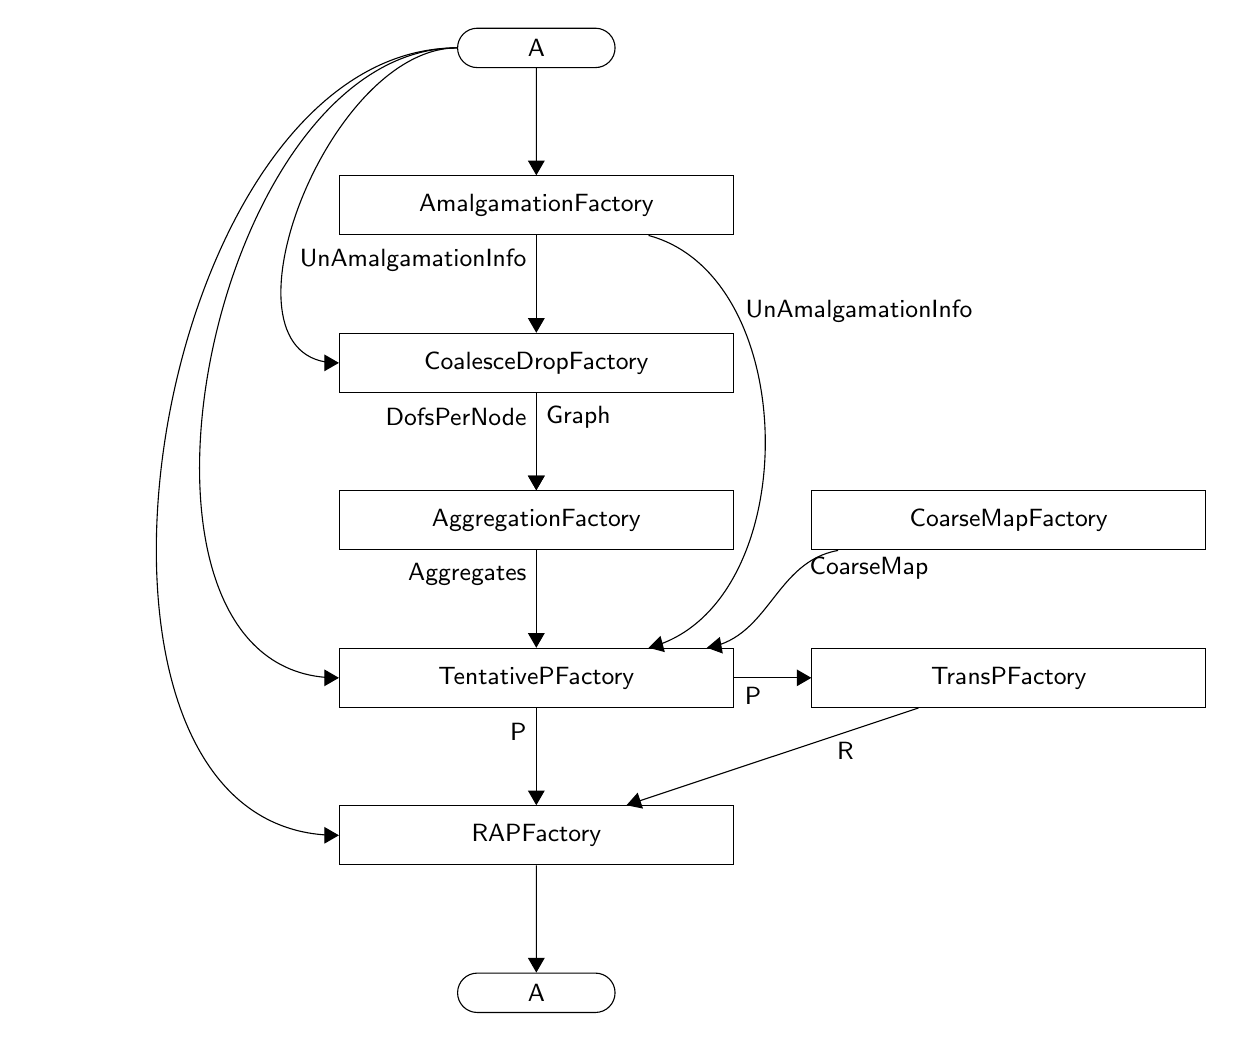
\begin{tikzpicture}[>=latex',font={\sf \small}, node distance=2cm]
\def\datawidth{2cm}
\def\dataheight{0.5cm}
\def\factorywidth{5cm}
\def\factoryheight{0.75cm}
%\draw[help lines] (-10,-10) grid (10,10);
\begin{scope}[>=triangle 60]
\node(A) at (-3,10) [draw, terminal, minimum width=\datawidth, minimum height=\dataheight]{A};
\node(AmalgamationFactory) at (-3,8) [draw, process, minimum width=\factorywidth, minimum height=\factoryheight]{AmalgamationFactory};
\node [draw, process, minimum width=\factorywidth, minimum height=\factoryheight, below of=AmalgamationFactory] (CoalesceDropFactory) {CoalesceDropFactory};
\node [draw, process, minimum width=\factorywidth, minimum height=\factoryheight, below of=CoalesceDropFactory] (AggregationFactory) {AggregationFactory};
\node [draw, process, minimum width=\factorywidth, minimum height=\factoryheight, below of=AggregationFactory] (TentativePFactory) {TentativePFactory};
\node [draw, process, minimum width=\factorywidth, minimum height=\factoryheight, right of=AggregationFactory,node distance=6cm] (CoarseMapFactory) {CoarseMapFactory};
\node [draw, process, minimum width=\factorywidth, minimum height=\factoryheight, right of=TentativePFactory,node distance=6cm] (TransPFactory) {TransPFactory};
\node [draw, process, minimum width=\factorywidth, minimum height=\factoryheight, below of=TentativePFactory] (RAPFactory) {RAPFactory};
\node(A2) at (-3,-2) [draw, terminal, minimum width=\datawidth, minimum height=\dataheight]{A};
\draw[->] (A) -- (AmalgamationFactory);
\draw[->] (AmalgamationFactory) -- node [near start, left] {UnAmalgamationInfo} (CoalesceDropFactory);
\draw[->] (AmalgamationFactory) to[out=-15,in=15] node [near start, right] {UnAmalgamationInfo} (TentativePFactory);
\draw[->] (CoalesceDropFactory) -- node [near start, left] {DofsPerNode} (AggregationFactory);
\draw[->] (CoalesceDropFactory) -- node [near start, right] {Graph} (AggregationFactory);
\draw[->] (A) to[out=180,in=180] node [near start, left] {} (CoalesceDropFactory);
\draw[->] (A) to[out=180,in=180] node [near start, left] {} (TentativePFactory);
\draw[->] (A) to[out=180,in=180] node [near start, left] {} (RAPFactory);
\draw[->] (AggregationFactory) -- node [near start, left] {Aggregates} (TentativePFactory);
\draw[->] (CoarseMapFactory) to[out=190,in=10] node [near start, right] {CoarseMap} (TentativePFactory);
\draw[->] (TentativePFactory) -- node [near start, below] {P} (TransPFactory);
\draw[->] (TentativePFactory) -- node [near start, left] {P} (RAPFactory);
\draw[->] (TransPFactory) -- node [near start, below] {R} (RAPFactory);
\draw[->] (RAPFactory) -- node [near start, below] {} (A2);
\end{scope}
\end{tikzpicture}
} % end scalebox

% symmetric design of 2x2 blocked preconditioner with repartitioning
\scalebox{0.6}{
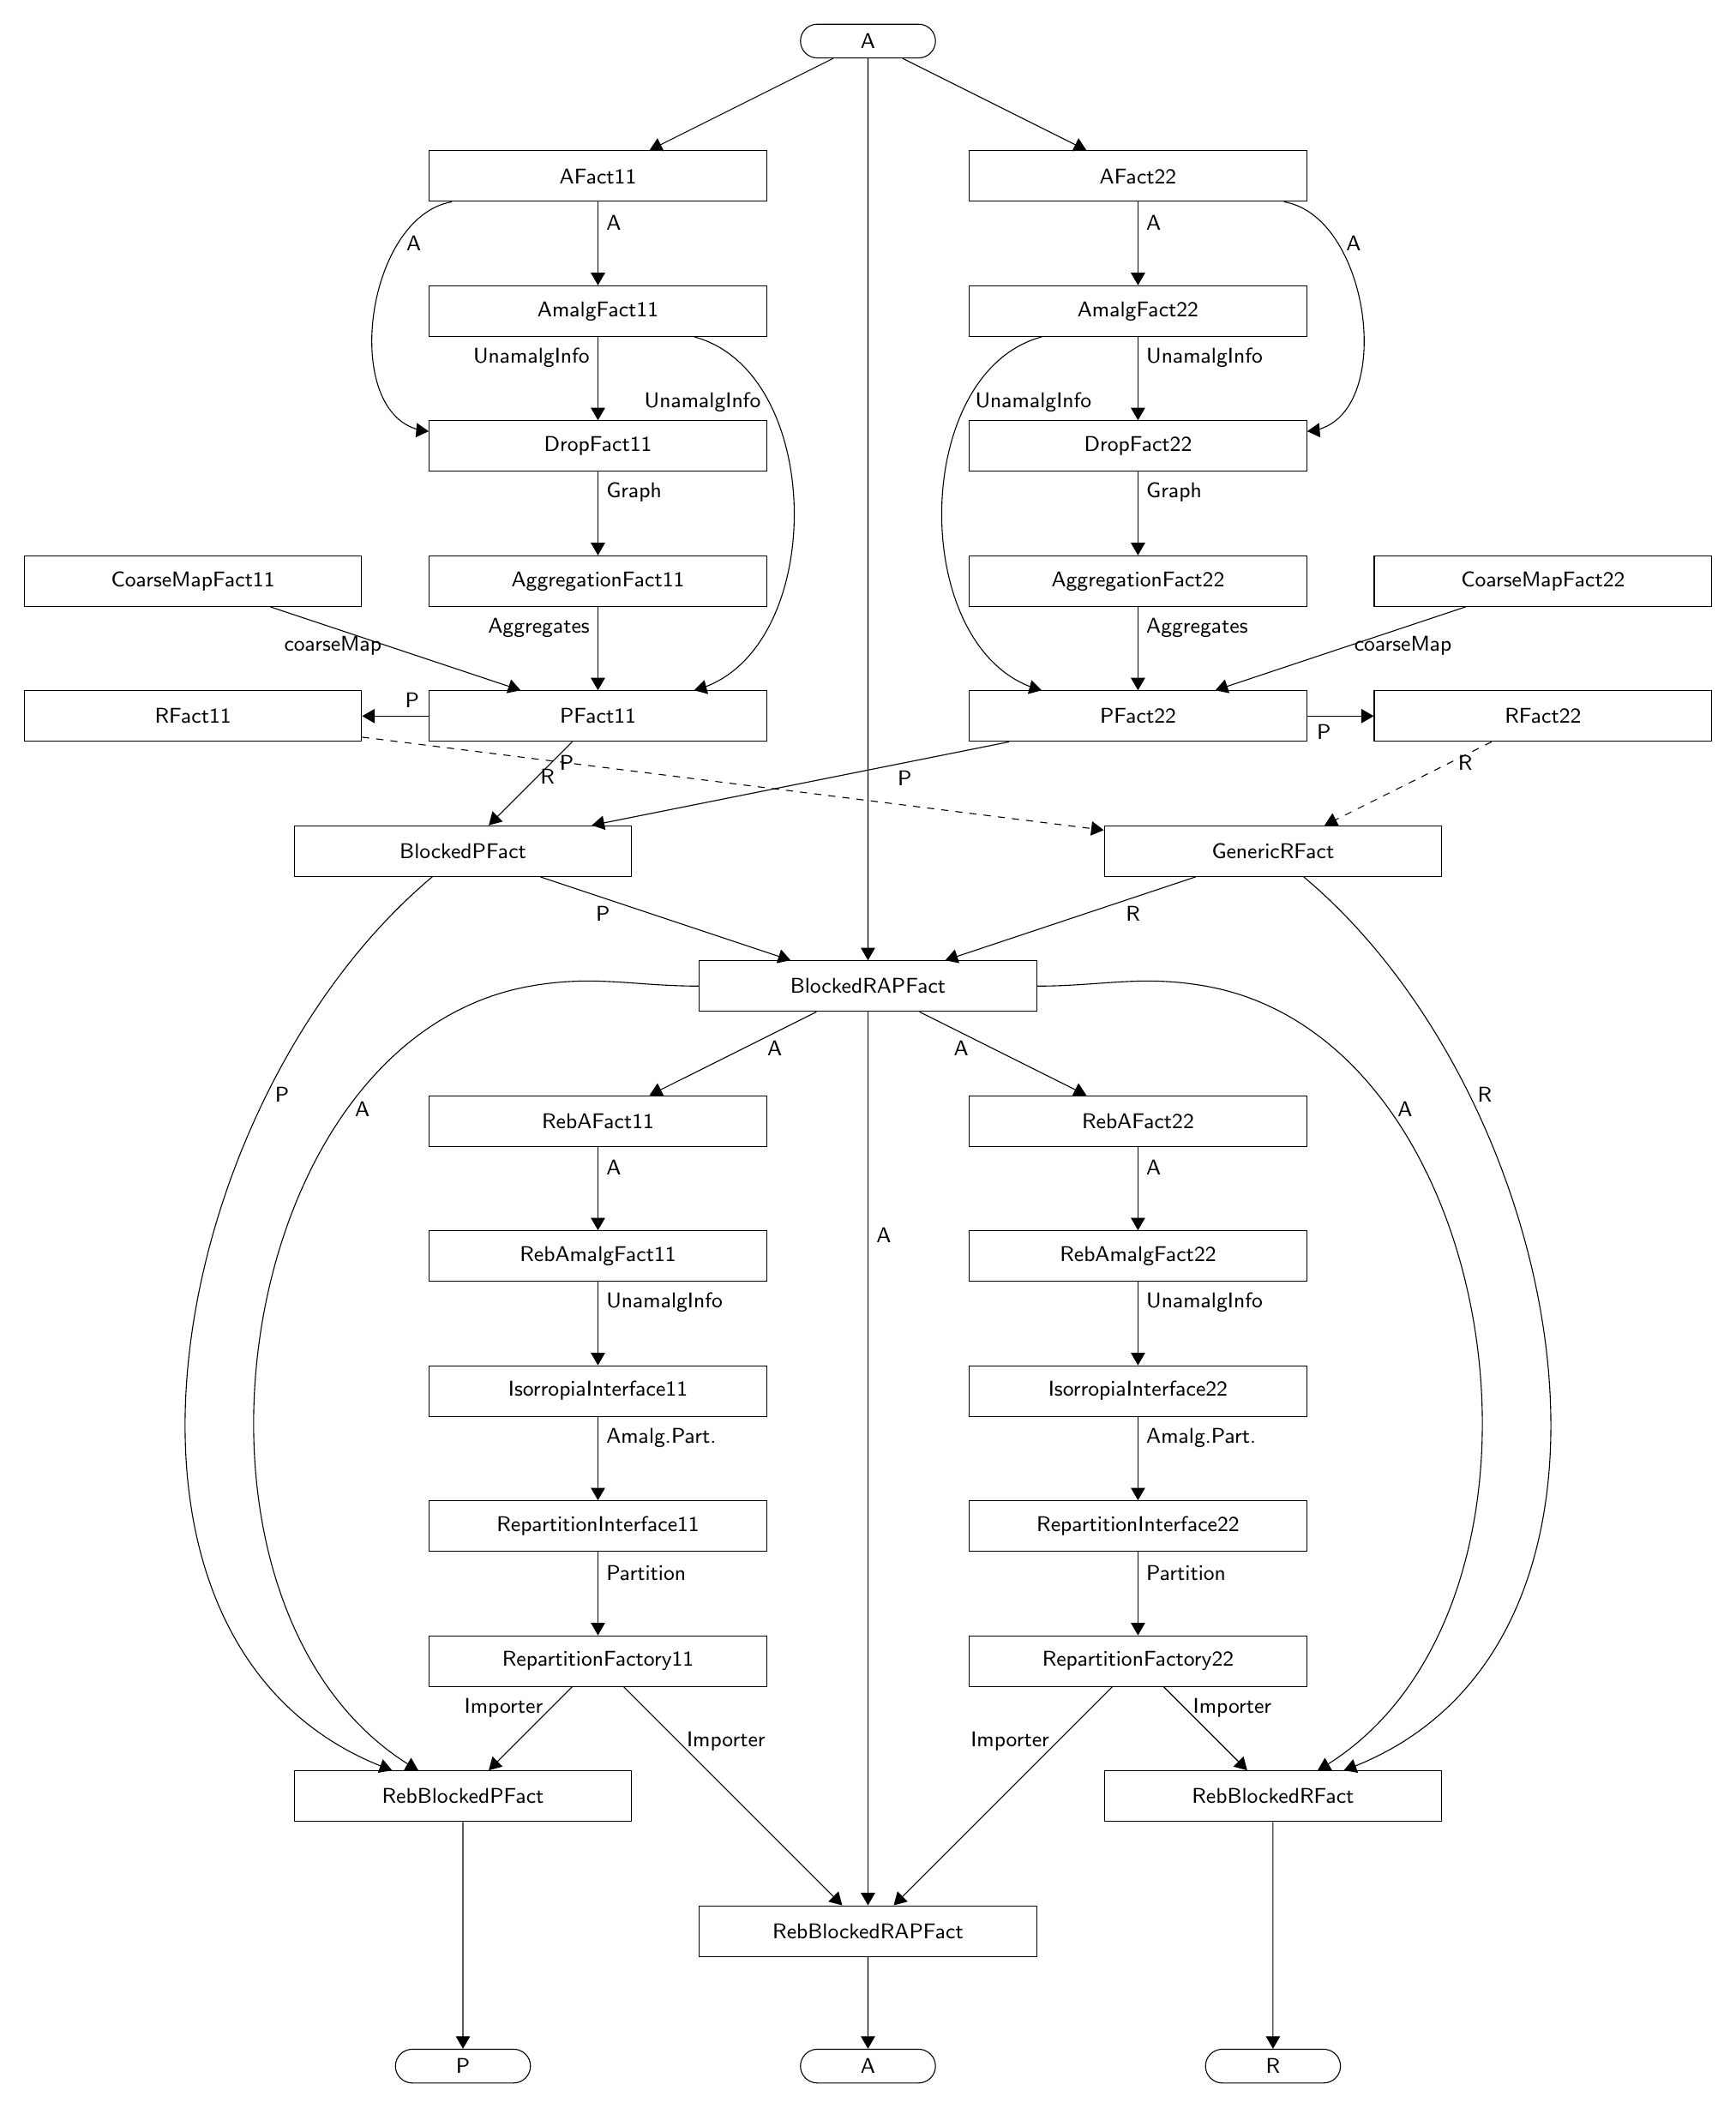
\begin{tikzpicture}[>=latex',font={\sf \small}, node distance=2cm]
\def\datawidth{2cm}
\def\dataheight{0.5cm}
\def\factorywidth{5cm}
\def\factoryheight{0.75cm}

%\draw[help lines] (-10,-10) grid (10,10);
\begin{scope}[>=triangle 60]
\node(A) at (1,10) [draw, terminal, minimum width=\datawidth, minimum height=\dataheight]{A};
\node(AFact11) at (-3,8) [draw, process, minimum width=\factorywidth, minimum height=\factoryheight]{AFact11};
\node [draw, process, minimum width=\factorywidth, minimum height=\factoryheight, below of=AFact11] (AmalgFact11) {AmalgFact11};
\node [draw, process, minimum width=\factorywidth, minimum height=\factoryheight, below of=AmalgFact11] (DropFact11) {DropFact11};
\node [draw, process, minimum width=\factorywidth, minimum height=\factoryheight, below of=DropFact11] (AggregationFact11) {AggregationFact11};
\node [draw, process, minimum width=\factorywidth, minimum height=\factoryheight, left of=AggregationFact11,node distance=6cm] (CoarseMapFact11) {CoarseMapFact11};
\node [draw, process, minimum width=\factorywidth, minimum height=\factoryheight, below of=AggregationFact11] (PFact11) {PFact11};
\node [draw, process, minimum width=\factorywidth, minimum height=\factoryheight, left of=PFact11,node distance=6cm] (RFact11) {RFact11};
\draw[->] (AFact11) -- node [near start, right] {A} (AmalgFact11);
\draw[->] (AFact11) to[out=190,in=175] node [near start, right] {A} (DropFact11);
\draw[->] (AmalgFact11) -- node [near start, left] {UnamalgInfo} (DropFact11);
\draw[->] (DropFact11) -- node [near start, right] {Graph} (AggregationFact11);
\draw[->] (AggregationFact11) -- node [near start, left] {Aggregates} (PFact11);
\draw[->] (PFact11) -- node [near start, above] {P} (RFact11);
\draw[->] (CoarseMapFact11) -- node [near start, below] {coarseMap} (PFact11);
\draw[->] (AmalgFact11) to[out=-15,in=15] node[near start, left] {UnamalgInfo} (PFact11);
\draw[->] (A) -- (AFact11);

\node [draw, process, minimum width=\factorywidth, minimum height=\factoryheight, right of=AFact11,node distance=8cm] (AFact22) {AFact22};
\node [draw, process, minimum width=\factorywidth, minimum height=\factoryheight, below of=AFact22] (AmalgFact22) {AmalgFact22};
\node [draw, process, minimum width=\factorywidth, minimum height=\factoryheight, below of=AmalgFact22] (DropFact22) {DropFact22};
\node [draw, process, minimum width=\factorywidth, minimum height=\factoryheight, below of=DropFact22] (AggregationFact22) {AggregationFact22};
\node [draw, process, minimum width=\factorywidth, minimum height=\factoryheight, right of=AggregationFact22,node distance=6cm] (CoarseMapFact22) {CoarseMapFact22};
\node [draw, process, minimum width=\factorywidth, minimum height=\factoryheight, below of=AggregationFact22] (PFact22) {PFact22};
\node [draw, process, minimum width=\factorywidth, minimum height=\factoryheight, right of=PFact22,node distance=6cm] (RFact22) {RFact22};
\draw[->] (AFact22) -- node [near start, right] {A} (AmalgFact22);
\draw[->] (AFact22) to[out=-10,in=5] node [near start, right] {A} (DropFact22);
\draw[->] (AmalgFact22) -- node [near start, right] {UnamalgInfo} (DropFact22);
\draw[->] (DropFact22) -- node [near start, right] {Graph} (AggregationFact22);
\draw[->] (AggregationFact22) -- node [near start, right] {Aggregates} (PFact22);
\draw[->] (PFact22) -- node [near start, below] {P} (RFact22);
\draw[->] (CoarseMapFact22) -- node [near start, below] {coarseMap} (PFact22);
\draw[->] (AmalgFact22) to[out=195,in=165] node[near start, right] {UnamalgInfo} (PFact22);
\draw[->] (A) -- (AFact22);

\node (BlockedPFact) at (-5,-2) [draw, process, minimum width=\factorywidth, minimum height=\factoryheight]  {BlockedPFact};
\node [draw, process, minimum width=\factorywidth, minimum height=\factoryheight, right of=BlockedPFact,node distance=12cm] (GenericRFact) {GenericRFact};
\draw[->] (PFact11) -- node [near start, right] {P} (BlockedPFact);
\draw[->] (PFact22) -- node [near start, below] {P} (BlockedPFact);
\draw[->,dashed] (RFact11) -- node [near start, below] {R} (GenericRFact);
\draw[->,dashed] (RFact22) -- node [near start, right] {R} (GenericRFact);

\node (BlockedRAPFact) at (1,-4) [draw, process, minimum width=\factorywidth, minimum height=\factoryheight]  {BlockedRAPFact};
\draw[->] (BlockedPFact) -- node [near start, below] {P} (BlockedRAPFact);
\draw[->] (GenericRFact) -- node [near start, below] {R} (BlockedRAPFact);
\draw[->] (A) -- (BlockedRAPFact);

\node (RebAFact11) at (-3,-6) [draw, process, minimum width=\factorywidth, minimum height=\factoryheight]  {RebAFact11};
\node [draw, process, minimum width=\factorywidth, minimum height=\factoryheight, below of=RebAFact11] (RebAmalgFact11) {RebAmalgFact11};
\node [draw, process, minimum width=\factorywidth, minimum height=\factoryheight, below of=RebAmalgFact11] (IsorropiaInterface11) {IsorropiaInterface11};
\node [draw, process, minimum width=\factorywidth, minimum height=\factoryheight, below of=IsorropiaInterface11] (RepartitionInterface11){RepartitionInterface11};
\node [draw, process, minimum width=\factorywidth, minimum height=\factoryheight, below of=RepartitionInterface11] (RepartitionFactory11) {RepartitionFactory11};


\node (RebAFact22) at (5,-6) [draw, process, minimum width=\factorywidth, minimum height=\factoryheight]  {RebAFact22};
\node [draw, process, minimum width=\factorywidth, minimum height=\factoryheight, below of=RebAFact22] (RebAmalgFact22) {RebAmalgFact22};
\node [draw, process, minimum width=\factorywidth, minimum height=\factoryheight, below of=RebAmalgFact22] (IsorropiaInterface22) {IsorropiaInterface22};
\node [draw, process, minimum width=\factorywidth, minimum height=\factoryheight, below of=IsorropiaInterface22] (RepartitionInterface22){RepartitionInterface22};
\node [draw, process, minimum width=\factorywidth, minimum height=\factoryheight, below of=RepartitionInterface22] (RepartitionFactory22) {RepartitionFactory22};

\node (RebBlockedPFact) at (-5,-16) [draw, process, minimum width=\factorywidth, minimum height=\factoryheight]  {RebBlockedPFact};
\node [draw, process, minimum width=\factorywidth, minimum height=\factoryheight, right of=RebBlockedPFact,node distance=12cm] (RebBlockedRFact) {RebBlockedRFact};
\node (RebBlockedRAPFact) at (1,-18) [draw, process, minimum width=\factorywidth, minimum height=\factoryheight]  {RebBlockedRAPFact};
\coordinate [left of=BlockedRAPFact,node distance=5cm](coLeftOfBlockedRAPFact);
\coordinate [right of=BlockedRAPFact,node distance=5cm](coRightOfBlockedRAPFact);
\draw[->] (BlockedRAPFact) -- node [near start, right] {A} (RebBlockedRAPFact);
\draw[->] (BlockedRAPFact) to[out=180,in=10] (coLeftOfBlockedRAPFact) to[out=190,in=150] node[near start, right] {A} (RebBlockedPFact);
\draw[->] (BlockedPFact) to[out=220,in=160] node [near start, right] {P} (RebBlockedPFact);

\draw[->] (BlockedRAPFact) to[out=0,in=170] (coRightOfBlockedRAPFact) to[out=-10,in=30] node[near start, right] {A} (RebBlockedRFact);
\draw[->] (GenericRFact) to[out=-40,in=20] node [near start, right] {R} (RebBlockedRFact);

\draw[->] (BlockedRAPFact) -- node [near start, below] {A} (RebAFact11);
\draw[->] (RebAFact11) -- node [near start, right] {A} (RebAmalgFact11);
\draw[->] (RebAmalgFact11) -- node [near start, right] {UnamalgInfo} (IsorropiaInterface11);
\draw[->] (IsorropiaInterface11) -- node [near start, right] {Amalg.Part.} (RepartitionInterface11);
\draw[->] (RepartitionInterface11) -- node [near start, right] {Partition} (RepartitionFactory11);
\draw[->] (RepartitionFactory11) -- node [near start, left] {Importer} (RebBlockedPFact);
\draw[->] (RepartitionFactory11) -- node [near start, right] {Importer} (RebBlockedRAPFact);

\draw[->] (BlockedRAPFact) -- node [near start, below] {A} (RebAFact22);
\draw[->] (RebAFact22) -- node [near start, right] {A} (RebAmalgFact22);
\draw[->] (RebAmalgFact22) -- node [near start, right] {UnamalgInfo} (IsorropiaInterface22);
\draw[->] (IsorropiaInterface22) -- node [near start, right] {Amalg.Part.} (RepartitionInterface22);
\draw[->] (RepartitionInterface22) -- node [near start, right] {Partition} (RepartitionFactory22);
\draw[->] (RepartitionFactory22) -- node [near start, right] {Importer} (RebBlockedRFact);
\draw[->] (RepartitionFactory22) -- node [near start, left] {Importer} (RebBlockedRAPFact);

\node [draw, terminal, minimum width=\datawidth, minimum height=\dataheight, below of=RebBlockedRAPFact](Acoarse){A};
\node [draw, terminal, minimum width=\datawidth, minimum height=\dataheight, below of=RebBlockedPFact, node distance=4cm](Pcoarse){P};
\node [draw, terminal, minimum width=\datawidth, minimum height=\dataheight, below of=RebBlockedRFact, node distance=4cm](Rcoarse){R};
\draw[->] (RebBlockedRAPFact) -- (Acoarse);
\draw[->] (RebBlockedPFact) -- (Pcoarse);
\draw[->] (RebBlockedRFact) -- (Rcoarse);
\end{scope}
\end{tikzpicture}
} % end scalebox

% non-symmetric design of 2x2 block preconditioner with reusing aggregates of upper-left block
\scalebox{0.6}{
\begin{tikzpicture}[>=latex',font={\sf \small}, node distance=2cm]
\def\datawidth{2cm}
\def\dataheight{0.5cm}
\def\factorywidth{5cm}
\def\factoryheight{0.75cm}

%\draw[help lines] (-10,-10) grid (10,10);
\begin{scope}[>=triangle 60]
\node(A) at (1,10) [draw, terminal, minimum width=\datawidth, minimum height=\dataheight]{A};
\node(AFact11) at (-3,8) [draw, process, minimum width=\factorywidth, minimum height=\factoryheight]{AFact11};
\node [draw, process, minimum width=\factorywidth, minimum height=\factoryheight, below of=AFact11] (AmalgFact11) {AmalgFact11};
\node [draw, process, minimum width=\factorywidth, minimum height=\factoryheight, below of=AmalgFact11] (DropFact11) {DropFact11};
\node [draw, process, minimum width=\factorywidth, minimum height=\factoryheight, below of=DropFact11] (AggregationFact11) {AggregationFact11};
\node [draw, process, minimum width=\factorywidth, minimum height=\factoryheight, left of=AggregationFact11,node distance=6cm] (CoarseMapFact11) {CoarseMapFact11};
\node [draw, process, minimum width=\factorywidth, minimum height=\factoryheight, below of=AggregationFact11] (PFact11) {PFact11};
\node [draw, process, minimum width=\factorywidth, minimum height=\factoryheight, left of=PFact11,node distance=6cm] (RFact11) {RFact11};
\draw[->] (AFact11) -- node [near start, right] {A} (AmalgFact11);
\draw[->] (AFact11) to[out=190,in=175] node [near start, right] {A} (DropFact11);
\draw[->] (AmalgFact11) -- node [near start, left] {UnamalgInfo} (DropFact11);
\draw[->] (DropFact11) -- node [near start, right] {Graph} (AggregationFact11);
\draw[->] (AggregationFact11) -- node [near start, left] {Aggregates} (PFact11);
\draw[->] (PFact11) -- node [near start, above] {P} (RFact11);
\draw[->] (CoarseMapFact11) -- node [near start, below] {coarseMap} (PFact11);
\draw[->] (AmalgFact11) to[out=-15,in=15] node[near start, left] {UnamalgInfo} (PFact11);
\draw[->] (A) -- (AFact11);

\node [draw, process, minimum width=\factorywidth, minimum height=\factoryheight, right of=AFact11,node distance=8cm] (AFact22) {AFact22};
\node [draw, process, minimum width=\factorywidth, minimum height=\factoryheight, below of=AFact22] (AmalgFact22) {AmalgFact22};
\node [draw, process, minimum width=\factorywidth, minimum height=\factoryheight, right of=AggregationFact22,node distance=6cm] (CoarseMapFact22) {CoarseMapFact22};
\node [draw, process, minimum width=\factorywidth, minimum height=\factoryheight, below of=AggregationFact22] (PFact22) {PFact22};
\node [draw, process, minimum width=\factorywidth, minimum height=\factoryheight, right of=PFact22,node distance=6cm] (RFact22) {RFact22};
\draw[->] (AFact22) -- node [near start, right] {A} (AmalgFact22);
\draw[->] (AmalgFact22) -- node [near start, right] {UnamalgInfo} (PFact22);
\draw[->] (PFact22) -- node [near start, below] {P} (RFact22);
\draw[->] (CoarseMapFact22) -- node [near start, below] {coarseMap} (PFact22);
\draw[->] (AggregationFact11) -- node [near end, above] {Aggregates} (PFact22);
\draw[->] (A) -- (AFact22);

\node (BlockedPFact) at (-5,-2) [draw, process, minimum width=\factorywidth, minimum height=\factoryheight]  {BlockedPFact};
\node [draw, process, minimum width=\factorywidth, minimum height=\factoryheight, right of=BlockedPFact,node distance=12cm] (GenericRFact) {GenericRFact};
\draw[->] (PFact11) -- node [near start, right] {P} (BlockedPFact);
\draw[->] (PFact22) -- node [near start, below] {P} (BlockedPFact);
\draw[->,dashed] (RFact11) -- node [near start, below] {R} (GenericRFact);
\draw[->,dashed] (RFact22) -- node [near start, right] {R} (GenericRFact);

\node (BlockedRAPFact) at (1,-4) [draw, process, minimum width=\factorywidth, minimum height=\factoryheight]  {BlockedRAPFact};
\draw[->] (BlockedPFact) -- node [near start, below] {P} (BlockedRAPFact);
\draw[->] (GenericRFact) -- node [near start, below] {R} (BlockedRAPFact);
\draw[->] (A) -- (BlockedRAPFact);

\node (RebAFact11) at (-3,-6) [draw, process, minimum width=\factorywidth, minimum height=\factoryheight]  {RebAFact11};
\node [draw, process, minimum width=\factorywidth, minimum height=\factoryheight, below of=RebAFact11] (RebAmalgFact11) {RebAmalgFact11};
\node [draw, process, minimum width=\factorywidth, minimum height=\factoryheight, below of=RebAmalgFact11] (IsorropiaInterface11) {IsorropiaInterface11};
\node [draw, process, minimum width=\factorywidth, minimum height=\factoryheight, below of=IsorropiaInterface11] (RepartitionInterface11){RepartitionInterface11};
\node [draw, process, minimum width=\factorywidth, minimum height=\factoryheight, below of=RepartitionInterface11] (RepartitionFactory11) {RepartitionFactory11};


\node (RebAFact22) at (5,-6) [draw, process, minimum width=\factorywidth, minimum height=\factoryheight]  {RebAFact22};
\node [draw, process, minimum width=\factorywidth, minimum height=\factoryheight, below of=RebAFact22] (RebAmalgFact22) {RebAmalgFact22};
\node [draw, process, minimum width=\factorywidth, minimum height=\factoryheight, below of=IsorropiaInterface22] (RepartitionInterface22){RepartitionInterface22};
\node [draw, process, minimum width=\factorywidth, minimum height=\factoryheight, below of=RepartitionInterface22] (RepartitionFactory22) {RepartitionFactory22};

\node (RebBlockedPFact) at (-5,-16) [draw, process, minimum width=\factorywidth, minimum height=\factoryheight]  {RebBlockedPFact};
\node [draw, process, minimum width=\factorywidth, minimum height=\factoryheight, right of=RebBlockedPFact,node distance=12cm] (RebBlockedRFact) {RebBlockedRFact};
\node (RebBlockedRAPFact) at (1,-18) [draw, process, minimum width=\factorywidth, minimum height=\factoryheight]  {RebBlockedRAPFact};
\coordinate [left of=BlockedRAPFact,node distance=5cm](coLeftOfBlockedRAPFact);
\coordinate [right of=BlockedRAPFact,node distance=5cm](coRightOfBlockedRAPFact);
\draw[->] (BlockedRAPFact) -- node [near start, right] {A} (RebBlockedRAPFact);
\draw[->] (BlockedRAPFact) to[out=180,in=10] (coLeftOfBlockedRAPFact) to[out=190,in=150] node[near start, right] {A} (RebBlockedPFact);
\draw[->] (BlockedPFact) to[out=220,in=160] node [near start, right] {P} (RebBlockedPFact);

\draw[->] (BlockedRAPFact) to[out=0,in=170] (coRightOfBlockedRAPFact) to[out=-10,in=30] node[near start, right] {A} (RebBlockedRFact);
\draw[->] (GenericRFact) to[out=-40,in=20] node [near start, right] {R} (RebBlockedRFact);

\draw[->] (BlockedRAPFact) -- node [near start, below] {A} (RebAFact11);
\draw[->] (RebAFact11) -- node [near start, right] {A} (RebAmalgFact11);
\draw[->] (RebAmalgFact11) -- node [near start, right] {UnamalgInfo} (IsorropiaInterface11);
\draw[->] (IsorropiaInterface11) -- node [near start, right] {Amalg.Part.} (RepartitionInterface11);
\draw[->] (RepartitionInterface11) -- node [near start, right] {Partition} (RepartitionFactory11);
\draw[->] (RepartitionFactory11) -- node [near start, left] {Importer} (RebBlockedPFact);
\draw[->] (RepartitionFactory11) -- node [near start, right] {Importer} (RebBlockedRAPFact);

\draw[->] (BlockedRAPFact) -- node [near start, below] {A} (RebAFact22);
\draw[->] (RebAFact22) -- node [near start, right] {A} (RebAmalgFact22);
\draw[->] (RebAmalgFact22) -- node [near start, right] {UnamalgInfo} (RepartitionInterface22);
\draw[->] (IsorropiaInterface11) -- node [near end, above] {Amalg.Part.} (RepartitionInterface22);
\draw[->] (RepartitionInterface22) -- node [near start, right] {Partition} (RepartitionFactory22);
\draw[->] (RepartitionFactory22) -- node [near start, right] {Importer} (RebBlockedRFact);
\draw[->] (RepartitionFactory22) -- node [near start, left] {Importer} (RebBlockedRAPFact);

\node [draw, terminal, minimum width=\datawidth, minimum height=\dataheight, below of=RebBlockedRAPFact](Acoarse){A};
\node [draw, terminal, minimum width=\datawidth, minimum height=\dataheight, below of=RebBlockedPFact, node distance=4cm](Pcoarse){P};
\node [draw, terminal, minimum width=\datawidth, minimum height=\dataheight, below of=RebBlockedRFact, node distance=4cm](Rcoarse){R};
\draw[->] (RebBlockedRAPFact) -- (Acoarse);
\draw[->] (RebBlockedPFact) -- (Pcoarse);
\draw[->] (RebBlockedRFact) -- (Rcoarse);
\end{scope}
\end{tikzpicture}
} % end scalebox
\end{document}